\documentclass{article}

\usepackage{iclr2026_conference,times}

\usepackage{amsmath}
\usepackage{amssymb}
\usepackage{amsthm}
\usepackage{mathtools}
\usepackage{nicefrac}
\usepackage{mathrsfs}
\usepackage{graphicx}
\usepackage{subcaption}
\usepackage[space]{grffile}
\usepackage{url}
\usepackage{booktabs}
\usepackage{float}
\usepackage{wrapfig}
\usepackage{algorithm}
\usepackage{algpseudocode}
\usepackage{hyperref}

\usepackage{glossaries}
\glsdisablehyper
\newacronym{ppo}{PPO}{Proximal Policy Optimization}
\newacronym{rtrl}{RTRL}{Real-Time Recurrent Learning}
\newacronym{rtd}{RTD($\lambda$)}{recurrent TD($\lambda$)}
\newacronym{rtu}{RTU}{Recurrent Trace Units}
\newacronym{gru}{GRU}{Gated Recurrent Unit}
\newacronym{lstm}{LSTM}{Long Short-Term Memory}
\newacronym{obgd}{ObGD}{Overshooting-bounded Gradient Descent}

\newtheorem{proposition}{Proposition}

\title{Streaming Reinforcement Learning under Partial Observability\\with Real-Time Recurrent Learning}

\author{Noah Farr\thanks{Equal contribution.}\ \ \thanks{Konrad Zuse School of Excellence in Learning and Intelligent Systems (ELIZA).}\\
Technical University of Darmstadt\\
\texttt{noah.farr@stud.tu-darmstadt.de}
\And
Aryaman Reddi\footnotemark[1]\\
Technical University of Darmstadt, University of W\"urzburg, Hessian.AI\\
\texttt{aryaman.reddi@tu-darmstadt.de}
\AND
Carlo D'Eramo\\
Technical University of Darmstadt, University of W\"urzburg, Hessian.AI
\And
Jan Peters\\
Technical University of Darmstadt, Hessian.AI, DFKI
}

\newcommand{\fix}{\marginpar{FIX}}
\newcommand{\new}{\marginpar{NEW}}

% \iclrfinalcopy  % uncomment for camera-ready / de-anonymised preprint

\renewcommand{\topfraction}{0.9}
\renewcommand{\bottomfraction}{0.7}
\renewcommand{\textfraction}{0.07}
\renewcommand{\floatpagefraction}{0.8}

\begin{document}

\maketitle

\begin{abstract}
We show that exact real-time recurrent learning (RTRL) over a diagonal recurrence composes with the eligibility trace of a streaming reinforcement learning update, giving streaming agents a credit horizon bounded by the slower of the trace decay and the retention of the recurrence. Streaming methods learn from one transition at a time with no replay buffer, which has kept partially observable tasks out of reach, since truncated backpropagation collapses to a one-step horizon in that setting and RTRL for general recurrent networks is quartic in the hidden size. Restricting to recurrences with a diagonal state-to-state Jacobian, satisfied by RTUs, minGRUs or any other diagonal state-space model, makes exact RTRL linear in the parameter count and lets it slot into any streaming algorithm built on a per-step gradient and an eligibility trace. The composition predicts which quantity sets the decay of credit under each gradient computation, and measurements on trained agents separate them, since lowering the trace decay moves the truncated weight and leaves the exact one where the retention puts it. On trace conditioning and MemoryChain exact RTRL tracks horizons up to four times longer than one-step truncation, and under the intentional update it solves chain length 256 at every trace decay we test, including the standard $0.8$ where the eligibility trace spans five steps, which one-step truncation reaches only as $\lambda$ approaches one. On eleven POPGym tasks the same agents beat their own memoryless counterparts on six to nine depending on the algorithm, and on masked MuJoCo they reach parity with recurrent PPO at matched capacity, indistinguishable on five of eight task-regime cells, once the trace decay is set for the recurrence rather than inherited from feedforward work.
\end{abstract}

\section{Introduction}
\label{sec:introduction}

We show that exact real-time recurrent learning (\gls{rtrl}) over a diagonal recurrence composes with the eligibility trace of a streaming reinforcement learning update, and that the composition sets the horizon over which a streaming agent can assign credit. Streaming agents update from each transition as it arrives, with no replay buffer and constant memory \citep{elsayed2024streaming, vasan2024deep}, but so far they have been confined to fully observable tasks, because backpropagation through time collapses to a one-step horizon, TBPTT(1), when there is no stored trajectory to unroll.

\gls{rtrl} \citep{williams1989learning} maintains the recurrent gradient forward in time and is the natural fit for streaming, but its cost is quartic in the hidden size for general recurrences. It becomes linear in the parameter count when the state-to-state Jacobian is diagonal, since each parameter then influences only its own unit. \gls{rtu}s \citep{elelimy2024real}, minGRUs \citep{feng2024were} and diagonal state-space models \citep{orvieto2023resurrecting} all satisfy this, where a \gls{gru} \citep{cho2014properties} or \gls{lstm} \citep{hochreiter1997long} does not. Prior work has trained such cells with \gls{ppo} \citep{schulman2017proximal, elelimy2024real} or with approximate forward-mode gradients inside a TD($\lambda$) actor-critic \citep{lemmel2025rtrrl}. We insert exact \gls{rtrl} into existing streaming algorithms unchanged and analyse the resulting update. The \gls{rtrl} sensitivity trace and the eligibility trace form one triangular linear system whose slower mode, the larger of the trace decay $\gamma\lambda$ and the retention $\rho$ of the recurrence, sets the rate at which credit on past steps decays, while TBPTT(1) decays at $\gamma\lambda$ alone.

The evidence is of three kinds. Measurements on trained agents show the truncated weight tracking $\gamma\lambda$ while the exact weight does not, and that retention is learned by minGRU but supplied by \gls{rtu}'s initialisation. On trace conditioning (Figure~\ref{fig:trace}) and MemoryChain, exact \gls{rtrl} tracks horizons up to four times longer than TBPTT(1), and on MemoryChain the reachable chain length grows with $\lambda$ under one-step truncation while exact \gls{rtrl} extends it further at every $\lambda$, by one grid step under RQRC($\lambda$) and to $L{=}256$ independently of $\lambda$ under the intentional update. On eleven POPGym tasks the recurrent agents beat the identical updates without a recurrence on six to nine depending on the algorithm, on masked MuJoCo they reach parity with recurrent \gls{ppo}, and on Foragax they keep relearning under a flipping reward. We do not claim state-of-the-art performance on any single benchmark.



\begin{figure}[t]
    \centering
    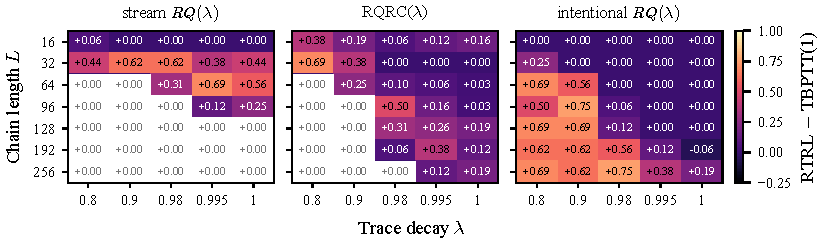
\includegraphics[width=0.84\linewidth]{plots/memory_chain/horizon_difference.pdf}
    \caption{Exact \gls{rtrl} helps most where the eligibility trace is short. Gain in solve rate
    over TBPTT(1) on MemoryChain against chain length $L$ and trace decay $\lambda$, for three
    streaming algorithms with a minGRU recurrence ($\gamma{=}0.999$, $16$--$32$ seeds per cell).
    A run is successful when its final return exceeds $0.5$. White cells are combinations
    neither method solves, as distinct from cells where both succeed and the gain is also zero.
    Appendix~\ref{sec:memory-chain-grids} gives the per-method rates.}
    \label{fig:memory_chain_lambda}
\end{figure}

\paragraph{Contributions.}
\begin{itemize}
    \item A proof that the \gls{rtrl} sensitivity trace and the eligibility trace form one
    triangular system whose slower mode bounds the credit horizon, with measured credit weights
    separating the two channels on trained agents.
    \item The consequence that horizon is not shared, since parameters reached by the sensitivity
    inherit the recurrence's retention, while the rest of the network decays at
    $\gamma\lambda$, so $\lambda$ remains consequential even when the recurrence retains for
    hundreds of steps. Neither $\lambda$ nor the streaming step-size rules transfer from
    feedforward work, and we show why, because the rules assume the trace is a decayed sum of recent
    gradients, which \gls{rtrl} violates in three distinct ways
    (Appendices~\ref{sec:lambda} and~\ref{sec:stepsize-analysis}).
    \item Streaming deep RL for partial observability with exact \gls{rtrl} over any
    diagonal-Jacobian recurrence, instantiated with \gls{rtu}s and minGRUs in five streaming
    algorithms, evaluated on trace conditioning, MemoryChain, POPGym, masked MuJoCo and
    continual foraging against recurrent \gls{ppo} at matched capacity, with a staleness bound
    for the sensitivity matrix under streaming updates in Appendix~\ref{sec:staleness-proof}.
\end{itemize}

\section{Background}
\label{sec:background}

\paragraph{Streaming reinforcement learning with eligibility traces.}
A streaming agent updates from each transition and discards it, and propagates credit across time with eligibility traces \citep{sutton1998introduction}. For a per-step gradient $\boldsymbol{g}_t$ of a value function or policy with respect to parameters $\boldsymbol{w}_t$,
\begin{equation}
    \boldsymbol{z}_t = \gamma\lambda \boldsymbol{z}_{t-1} + \boldsymbol{g}_t, \qquad \boldsymbol{w}_{t+1} = \boldsymbol{w}_t + \alpha \delta_t \boldsymbol{z}_t, \qquad \boldsymbol{z}_0 \doteq \boldsymbol{0},
\end{equation}
where $\delta_t$ is the TD error, $\alpha$ the step size and $\lambda \in [0,1]$ the trace decay. Existing streaming deep RL methods \citep{elsayed2024streaming, vasan2024deep} use feedforward function approximation, where $\boldsymbol{g}_t$ is the backpropagated gradient of a single sample.

\paragraph{Real-time recurrent learning.}
For a recurrent network $\boldsymbol{h}_t = \boldsymbol{f}(\boldsymbol{h}_{t-1}, \boldsymbol{x}_t; \boldsymbol{\psi})$ with parameters
$\boldsymbol{\psi}$, computing $\boldsymbol{g}_t$ requires the gradient
$\partial \boldsymbol{h}_t / \partial \boldsymbol{\psi}$ of the current hidden state with respect to
the recurrent parameters. Backpropagation through time (BPTT) obtains this gradient by unrolling the recurrence backward over a stored trajectory of length $T$, which reduces to a one-step gradient horizon when $T=1$. \gls{rtrl}
\citep{williams1989learning} avoids this unrolling by maintaining the gradient forward through time, applying the chain rule to the recurrence,
\begin{equation}
    \frac{\partial \boldsymbol{h}_t}{\partial \boldsymbol{\psi}}
    = \frac{\partial \boldsymbol{f}(\boldsymbol{h}_{t-1},\boldsymbol{x}_t; \boldsymbol{\psi})}{\partial \boldsymbol{\psi}}
    + \frac{\partial \boldsymbol{f}(\boldsymbol{h}_{t-1},\boldsymbol{x}_t; \boldsymbol{\psi})}{\partial \boldsymbol{h}_{t-1}} \,
      \frac{\partial \boldsymbol{h}_{t-1}}{\partial \boldsymbol{\psi}}.
\end{equation}
The first term is the direct dependence of $\boldsymbol{h}_t$ on $\boldsymbol{\psi}$ through the
current step. The second propagates accumulated dependence through
$\boldsymbol{h}_{t-1}$. For a general recurrent network with hidden dimension $n$ and
parameter count $O(n^2)$, this gradient is an $n \times O(n^2)$ matrix
and the recursion costs $O(n^4)$ per step, prohibitive even for moderate
$n$.

\paragraph{Diagonal recurrences.}
Exact \gls{rtrl} is expensive because it carries a dense influence matrix through a dense
state-to-state Jacobian $\boldsymbol{J}_t$. When $\boldsymbol{J}_t$ is diagonal each hidden unit
feeds only itself, the recursion decouples, and the cost falls to
$\mathcal{O}(|\boldsymbol{\psi}|)$ per step rather than quartic in the hidden size. This depends
on the Jacobian alone, so it holds across the diagonal state-space family however the diagonal is
parameterised. We take two instances that put the retention in different places.

\gls{rtu}s \citep{elelimy2024real} use a linear diagonal complex-valued recurrence,
\begin{equation}
    \boldsymbol{h}_t = \boldsymbol{\Lambda} \boldsymbol{h}_{t-1} + \boldsymbol{W} \boldsymbol{x}_t,
\end{equation}
where $\boldsymbol{\Lambda} \in \mathbb{C}^{n\times n}$ is diagonal with entries
$\lambda_k = r_k(\cos\Omega_k + i\sin\Omega_k)$, where $r_k$ and $\Omega_k$ define the polar
complex representation of the $k$'th parameter, so $\boldsymbol{J}_t$ is constant in the input.
Figure~\ref{fig:rtrl} in Appendix~\ref{sec:memory-chain-extra} confirms the linear cost.

The minGRU \citep{feng2024were} meets the same condition with a real gate rather than a
complex rotation, $\boldsymbol{h}_t = (\boldsymbol{1}-\boldsymbol{u}_t) \odot \boldsymbol{h}_{t-1}
+ \boldsymbol{u}_t \odot \boldsymbol{W}_h \boldsymbol{x}_t$ with
$\boldsymbol{u}_t = \sigma(\boldsymbol{W}_u \boldsymbol{x}_t)$ depending on the input alone, so
$\boldsymbol{J}_t = \mathrm{diag}(\boldsymbol{1}-\boldsymbol{u}_t)$ varies with the input while
staying diagonal. The two differ in where retention comes from, \gls{rtu}'s $r_k$
being set near one at initialisation while the minGRU gate starts at $0.5$ and must raise it,
and in how credit accumulates, since a real positive retention adds terms that cannot cancel
while \gls{rtu}'s complex rotation can interfere destructively across lags
(Section~\ref{sec:weights}).



\section{Methodology}
\label{sec:methodology}


Our method makes a single change to existing streaming algorithms.
Where an algorithm typically uses a feedforward function approximator
mapping observations to values or actions, we insert a diagonal recurrent layer between the observation and the feedforward head. The streaming machinery, including eligibility traces and step-size
adaptation, is unchanged, and the only modification is how the per-step gradient feeding the
trace is computed. Figure~\ref{fig:architecture} shows the data flow.



\paragraph{Per-step gradient.}
The function approximator has three parameter groups, an encoder
$\phi(\,\cdot\,;\boldsymbol{\theta})$ producing features $\boldsymbol{x}_t$, a diagonal recurrent
layer with parameters $\boldsymbol{\psi}$ producing the state
$\boldsymbol{h}_t$, and a feedforward head with parameters $\boldsymbol{w}$, for instance a
value head $v(\boldsymbol{h}_t; \boldsymbol{w}_v)$. We compute the gradient
of the head output with respect to each group in a single backward pass,
combined with the layer's forward-mode \gls{rtrl} trace
$\boldsymbol{S}_t = \partial \boldsymbol{h}_t / \partial \boldsymbol{\psi}$.

The head parameters have no temporal dependency and receive an ordinary
backward pass. The recurrent parameters enter only through
$\boldsymbol{h}_t$, so combining the backward pass through the head with
$\boldsymbol{S}_t$ yields their gradient across the entire history at
$\mathcal{O}(|\boldsymbol{\psi}|)$ per step. The encoder parameters influence the state both
instantaneously through $\boldsymbol{x}_t$ and recursively through every past state, and an
exact trace for them would cost
$\mathcal{O}(|\boldsymbol{\theta}|\cdot\dim \boldsymbol{h})$ per step, prohibitive for a deep
encoder. We therefore backpropagate through the head, a single step of the recurrence and the
encoder, which credits the encoder for its immediate effect on $\boldsymbol{h}_t$ while ignoring
its influence through past states.

\paragraph{Composition with eligibility traces.}
Operationally the two traces compose without modification. The \gls{rtrl} trace is a
forward-mode object that maintains $\partial \boldsymbol{h}_t / \partial \boldsymbol{\psi}$ at
each step, and the eligibility trace is a temporal accumulator of whatever per-step gradient the
streaming algorithm supplies. Each recurrent layer hands over its sensitivity on demand and the
eligibility trace folds it into the usual recursion.

Their effects on credit assignment, however, are not independent. The bound below governs how
credit is weighted, not whether any is available to assign.
Appendix~\ref{sec:composition-caveats} gives three qualifications, including why $\lambda$ is not
free and why $\rho > \gamma\lambda$ is the typical case.

\begin{proposition}
\label{prop:composition}
Write $\boldsymbol{J}_t = \partial \boldsymbol{h}_t / \partial \boldsymbol{h}_{t-1}$ for the
state-to-state Jacobian and
$\boldsymbol{I}_t = \partial \boldsymbol{h}_t / \partial \boldsymbol{\psi}$ for the immediate
Jacobian, the one-step part of the full sensitivity $\boldsymbol{S}_t$. Let
$\boldsymbol{c}_t^\top = \partial v(\boldsymbol{h}_t;\boldsymbol{w}_v) / \partial \boldsymbol{h}_t$
be the head's sensitivity to the state. Let
$\boldsymbol{\Phi}_{i,k} \doteq \boldsymbol{J}_i \boldsymbol{J}_{i-1}\cdots\boldsymbol{J}_{k+1}$
for $i > k$, with $\boldsymbol{\Phi}_{k,k}$ the identity.
At the end of an episode of length $T$ the eligibility trace is a weighted sum over the same
immediate Jacobians under either gradient computation,
$\boldsymbol{z}_T = \sum_{k=0}^{T} \boldsymbol{\omega}_k \boldsymbol{I}_k$, so the two differ only
in their weights,
\begin{equation}
    \boldsymbol{\omega}_k^{\mathrm{TBPTT(1)}} = (\gamma\lambda)^{T-k}\, \boldsymbol{c}_k^\top,
    \qquad
    \boldsymbol{\omega}_k^{\mathrm{\gls{rtrl}}}
    = \sum_{i=k}^{T} (\gamma\lambda)^{T-i}\, \boldsymbol{c}_i^\top \boldsymbol{\Phi}_{i,k}.
\end{equation}
Exact \gls{rtrl} keeps the terms with $i > k$, which carry the dependence of later states on
$\boldsymbol{h}_k$. Writing $\rho \doteq \max_t \|\boldsymbol{J}_t\|$ and
$C \doteq \max_t \|\boldsymbol{c}_t\|$,
\begin{equation}
    \|\boldsymbol{\omega}_k^{\mathrm{\gls{rtrl}}}\|
    \;\le\; C \sum_{i=k}^{T} (\gamma\lambda)^{T-i} \rho^{\,i-k}
    \;=\; \mathcal{O}\!\left(\max(\gamma\lambda,\rho)^{\,T-k}\right)
\end{equation}
for $\rho \neq \gamma\lambda$. At equality all $T-k+1$ terms have the same size and the bound
gains a factor $T-k+1$.
\end{proposition}

Substituting the \gls{rtrl} recursion into the eligibility trace shows why. The pair
$(\boldsymbol{S}_t, \boldsymbol{z}_t)$ evolves as one block-triangular linear system whose modes
are those of the recurrence together with $\gamma\lambda$, and TBPTT(1) severs the coupling
between them, so the decay is bounded by whichever mode is slower. Writing $n = T-k$ for the lag,
the ratio of the two weights on the same immediate Jacobian separates into two regimes,
\begin{equation}
    \frac{\|\boldsymbol{\omega}_k^{\mathrm{\gls{rtrl}}}\|}
         {\|\boldsymbol{\omega}_k^{\mathrm{TBPTT(1)}}\|}
    \;\sim\;
    \begin{cases}
        n + 1, & \rho \approx \gamma\lambda, \\[4pt]
        \left(\dfrac{\rho}{\gamma\lambda}\right)^{\!n}, & \rho > \gamma\lambda,
    \end{cases}
    \label{eq:amplification}
\end{equation}
since the geometric sum collapses to $n+1$ equal terms when the modes coincide and is dominated
by its last otherwise. Exact \gls{rtrl} therefore amplifies distant credit, linearly in the lag
when $\rho \approx \gamma\lambda$, exponentially when $\rho > \gamma\lambda$, and at no better
rate when $\rho < \gamma\lambda$.


\begin{table}[t]
\centering
\caption{Decay of the credit weight $\|\boldsymbol{\omega}_k\|$ with lag on trained MemoryChain
agents, $L{=}64$ and medians over $10$ seeds, against the rates of
Proposition~\ref{prop:composition}, $\gamma\lambda$ for TBPTT(1) and $\max(\gamma\lambda,\rho)$
for \gls{rtrl} with $\rho$ the measured retention. The last column is the amplification of exact
\gls{rtrl} over TBPTT(1) at lag $32$.}
\label{tab:weights}
\small
\setlength{\tabcolsep}{3.8pt}
\begin{tabular}{llllccc}
\toprule
Cell & $\lambda$ & $\gamma\lambda$ & $\rho$ &
$\|\boldsymbol{\omega}^{\mathrm{TBPTT(1)}}\|^{1/n}$ &
$\|\boldsymbol{\omega}^{\mathrm{\gls{rtrl}}}\|^{1/n}$ &
$\nicefrac{\|\boldsymbol{\omega}^{\mathrm{\gls{rtrl}}}\|}{\|\boldsymbol{\omega}^{\mathrm{TBPTT(1)}}\|}$ \\
\midrule
minGRU & $1$    & $0.999$ & $0.9993$ & $0.9995$ & $1.0140$ & $20.1$ \\
minGRU & $0.98$ & $0.979$ & $0.9995$ & $0.9791$ & $0.9942$ & $33.2$ \\
\gls{rtu}    & $1$    & $0.999$ & $0.9989$ & $0.9972$ & $1.0193$ & $6.4$ \\
\gls{rtu}    & $0.98$ & $0.979$ & $0.9989$ & $0.9786$ & $1.0007$ & $9.2$ \\
\bottomrule
\end{tabular}
\end{table}

\paragraph{The two channels separate in measurement.}
\label{sec:weights}
We freeze trained agents and measure $\|\boldsymbol{\omega}_k\|$ against lag on MemoryChain at
$L{=}64$, with medians over 10 seeds. Table~\ref{tab:weights} reports the fitted rates. The
TBPTT(1) weight tracks $\gamma\lambda$ at both trace decays, while the \gls{rtrl} weight stays
near one and barely moves when $\lambda$ drops, since the recurrence retains what the trace
discards. That places it in the near-degenerate regime $\rho \approx \gamma\lambda$, so
\eqref{eq:amplification} orders the two channels without being tight on either. The
amplification at lag $32$ spans one to one and a half orders of magnitude and is cell-dependent,
larger for minGRU than for \gls{rtu}, which the same measurements attribute to phase
cancellation under \gls{rtu}'s complex rotation.
Appendix~\ref{sec:credit-appendix} gives the protocol, the per-lag measurements and the
effect of exploration cuts, which favour \gls{rtrl} because zeroing the eligibility trace on a
non-greedy action leaves the influence matrix intact.

\paragraph{Instantiations.} We evaluate on five streaming algorithms covering prediction,
value-based control and policy-based control, namely stream TD($\lambda$), stream Q($\lambda$) and
stream AC($\lambda$) \citep{elsayed2024streaming}, QRC($\lambda$) \citep{elelimy2025deep} and
intentional Q($\lambda$) \citep{sharifnassab2026intentional}. We call their recurrent instances
stream RTD($\lambda$), stream RQ($\lambda$), stream RAC($\lambda$), RQRC($\lambda$) and
intentional RQ($\lambda$), and the TBPTT(1) ablations use the same networks with the one-step
gradient.
Stream RTD($\lambda$) is applied to trace conditioning, the three value-based algorithms to
MemoryChain and POPGym, and stream
RAC($\lambda$) and intentional RAC($\lambda$) to masked MuJoCo. Each network carries its own recurrent layer and \gls{rtrl} trace, so their recurrent
parameters are updated independently. Appendix~\ref{sec:pseudocode} gives pseudocode.

\section{Experiments}
\label{sec:experiments}
 
We evaluate the method on five benchmarks chosen to isolate distinct properties, and on a sixth in Appendix~\ref{sec:staleness}.
Trace conditioning (Section~\ref{sec:trace}) tests the credit horizon on pure prediction, and MemoryChain (Section~\ref{sec:memory_chain}) sweeps it under control.
POPGym (Section~\ref{sec:popgym}) tests whether the streaming method is competitive with a recurrent baseline that reuses each transition, on long-memory discrete control.
Masked MuJoCo (Section~\ref{sec:mujoco}) extends the evaluation to continuous control.
Foragax (Section~\ref{sec:foragax}) tests continual relearning under a periodically inverted reward.
All curves report the interquartile mean (IQM) with shaded standard error, and seed counts vary by experiment and are stated in each caption. The recurrence is not held constant. MemoryChain uses minGRU, which reaches longer chains there than \gls{rtu} does, because real positive retentions accumulate coherently where a complex rotation cancels, the same effect Section~\ref{sec:weights} measures. Elsewhere the body figures use \gls{rtu}, while trace conditioning, POPGym and Foragax each report minGRU and a memoryless network alongside it, the POPGym repeats in Appendix~\ref{sec:popgym-cells}. Only masked MuJoCo leaves the cell and the benchmark confounded.
Hyperparameters, network architectures, and per-task details are listed in Appendix \ref{sec:hyperparameters}.
 
\subsection{Trace conditioning}
\label{sec:trace}

Exact \gls{rtrl} tracks interstimulus intervals that one-step truncation cannot, and $\lambda$ matters far more for the truncated update than for the exact one.

\begin{figure}[t]
    \centering
    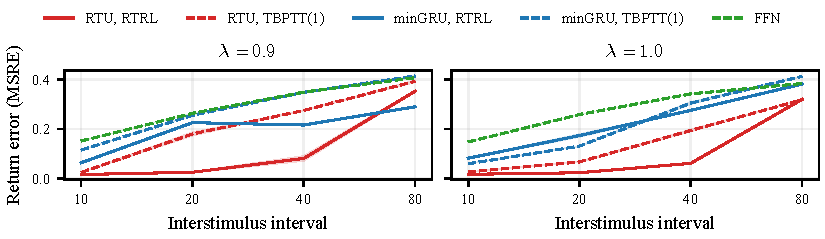
\includegraphics[width=\linewidth]{plots/trace_conditioning/return_error.pdf}
    \caption{Return error on trace conditioning against the interstimulus interval, IQM with standard error over 10 seeds, for stream RTD($\lambda$) under exact \gls{rtrl} (solid) and TBPTT(1) (dashed) at $\lambda{=}0.9$ and $\lambda{=}1$, with $\gamma$ per ISI as in \citet{rafiee2022eye}. At $\lambda{=}0.9$ exact \gls{rtrl} with \gls{rtu} tracks the timing where TBPTT(1) falls to the memoryless baseline, and at $\lambda{=}1$ the trace carries TBPTT(1) most of the way (Section~\ref{sec:trace}).}
    \label{fig:trace}
\end{figure}

\paragraph{Task and design.}
Trace conditioning \citep{rafiee2022eye} is a prediction task, where a conditioned stimulus precedes an unconditioned one by an interstimulus interval (ISI), and the agent observes both and predicts the discounted sum of the unconditioned stimulus, with $\gamma$ set per ISI as in the original benchmark so that $1/(1-\gamma)$ matches the ISI. This is the setting of Proposition~\ref{prop:composition}, namely prediction under a fixed behaviour, with the memory length set by the ISI. We run stream RTD($\lambda$) with \gls{rtu}, minGRU and a memoryless network for 2M steps and 10 seeds and report the mean squared error of the prediction against the true return.


\paragraph{Result.}
Figure~\ref{fig:trace} shows that \gls{rtu} under exact \gls{rtrl} is the only configuration that tracks the timing beyond ISI 10: at ISI 20 and 40 its error is $5.1\times$ and $3.1\times$ below TBPTT(1) at $\lambda{=}0.9$, where TBPTT(1) sits near the memoryless baseline. Raising $\lambda$ to $1$ helps TBPTT(1) substantially ($0.18$ to $0.07$ at ISI 20), which is the
eligibility trace extending the horizon. Exact \gls{rtrl} moves less but not negligibly, since at ISI
40 its error falls from $0.090$ at $\lambda{=}0.9$ to $0.059$ at $0.95$, rising again to $0.064$
at $0.99$ and $1$, so an interior optimum exists here as it does on masked MuJoCo, at a
different $\lambda$ (Appendix~\ref{sec:lambda}). At ISI 80 the recurrent configurations are at
best level with the memoryless baseline within 2M steps, several of them sitting just below it
in error, and minGRU trails \gls{rtu} at every ISI except $80$.

\subsection{MemoryChain}

The solvable chain length grows with the trace decay under TBPTT(1). Exact \gls{rtrl} reaches further at every decay, and under the intentional update it stops depending on the decay at all.
\label{sec:memory_chain}
 
\paragraph{Task and design.}
The MemoryChain~\citep{osband2020bsuite} task presents an informative binary cue at $t{=}0$.
The agent then receives uninformative observations for $L{-}1$ steps and is rewarded for reproducing the cue at $t{=}L$.
The chain length $L$ controls how far back the agent must propagate credit, isolating the temporal credit-assignment problem from representation learning.
We sweep the chain length and the trace decay jointly, $L \in \{16, 32, 64, 96, 128, 192,
256\}$ against $\lambda \in \{0.8, 0.9, 0.98, 0.995, 1\}$, and run all three streaming
algorithms, stream RQ($\lambda$), RQRC($\lambda$)~\citep{elelimy2025deep} and intentional
RQ($\lambda$), each with a minGRU recurrence under exact \gls{rtrl} and under TBPTT(1), at
$\gamma{=}0.999$ with $16$--$32$ seeds per cell. A run counts as successful when its final
return exceeds $0.5$, and all non-recurrence hyperparameters are matched across agents.
 




\paragraph{The trace decay controls this gap.}
Proposition~\ref{prop:composition} predicts that this comparison is specific to the regime
$\rho > \gamma\lambda$, since the eligibility trace and the \gls{rtrl} trace carry credit in
parallel and the slower mode dominates. At $\lambda{=}0.8$ and $\gamma{=}0.999$ the trace mode
decays with an effective horizon of roughly five steps, which is consistent with the collapse
observed past $L{=}16$, leaving the recurrent gradient as the only channel. Raising $\lambda$ to
one removes that limit, and Figure~\ref{fig:memory_chain_lambda} sweeps both quantities jointly.
Section~\ref{sec:weights} measures
$\rho \approx 0.999$ on this task, a retention horizon of roughly a thousand steps and longer
than any chain in the sweep, so the prediction is that the TBPTT(1) boundary moves with
$\lambda$ while the \gls{rtrl} boundary need not.
Under RQRC($\lambda$) the longest chain TBPTT(1) solves on a majority of seeds grows with the
trace horizon $(1-\gamma\lambda)^{-1}$, from $L{=}16$ at $\lambda{=}0.8$ to $L{=}128$ at
$\lambda{=}0.995$, though sublinearly, since the ratio $L/(1-\gamma\lambda)^{-1}$ falls from
$3.2$ to $0.77$ across the sweep. Exact \gls{rtrl} moves that boundary one grid step deeper at every
$\lambda$ but one, and its advantage is largest along the boundary, reaching $0.69$ at
$L{=}32,\lambda{=}0.8$. The advantage vanishes in two limits the figure keeps distinct, since at high
$\lambda$ the trace already spans the episode and the two channels coincide, while at long $L$
neither method succeeds.

The ordering is algorithm-independent and the reachable horizon is not. Exact \gls{rtrl} is at
least as good as TBPTT(1) in every cell of all three grids but one, with mean gains of $+0.13$,
$+0.14$ and $+0.25$, while the absolute reach differs by an order of magnitude. Stream
RQ($\lambda$) never passes $L{=}64$, whereas under intentional RQ($\lambda$) exact \gls{rtrl}
solves $L{=}256$ at every $\lambda$ including $0.8$, where the trace spans five steps. That
$\lambda$-independence is what Proposition~\ref{prop:composition} predicts for the \gls{rtrl}
channel once $\rho$ exceeds $\gamma\lambda$. The spread tracks the retention each algorithm
learns, $0.981$, $0.999$ and $0.99995$ respectively, ordered exactly as their reachable horizons
are. It is not
sufficient, however, since the credit horizon $(1-\rho)^{-1}$ exceeds the observed boundary in every
cell of every grid, by factors from $1.5$ to nearly $400$. The choice of cell matters
independently of the gradient method, and freezing the recurrence at initialisation solves
$L{=}16$ and nothing beyond $L{=}32$. Appendix~\ref{sec:memory-chain-grids} gives the full
grids, the per-cell gains and the frozen control.

\subsection{POPGym}

The recurrence earns its place on six to nine of eleven tasks depending on the algorithm, and the streaming methods trail recurrent \gls{ppo} on eight of eleven, where reusing transitions pays. Masked MuJoCo reaches parity once the trace decay is set for the recurrence.
\label{sec:popgym}
 
\paragraph{Task and design.}
We evaluate on eleven tasks from the POPGym Easy suite~\citep{morad2023popgym}:
Autoencode, Battleship, Concentration, CountRecall, HigherLower, MineSweeper,
MultiArmedBandit, NoisyStatelessCartPole, RepeatFirst, RepeatPrevious, and
StatelessCartPole.
We compare three streaming value-based methods, stream RQ($\lambda$), RQRC($\lambda$)
and intentional RQ($\lambda$), each paired with \gls{rtu}, against a recurrent
\gls{ppo}-\gls{rtu} baseline in the real-time design of \citet{elelimy2024real}, which
stores the \gls{rtrl} sensitivity of every rollout step and updates on single-step
minibatches, so every sample carries an exact recurrent gradient. It uses the same
recurrence without the streaming constraint.
Each agent is run for 10M environment frames with 10 seeds, and we report the
interquartile mean with shaded standard error.
Returns are normalised per task so that $0$ is the minimum episodic return and $1$ the return
of an optimal policy, which puts the panels on a common scale.
\paragraph{Memoryless ceiling.}
POPGym aliases the previous action into the observation, so a memoryless agent sees
$(o_t, a_{t-1})$. Each algorithm is plotted twice, solid with an \gls{rtu} recurrence and dashed with a
feedforward network (FFN), at the same budget and seed count, so every comparison is against the
identical update with the recurrence removed. Bootstrapping that difference at 10M frames, the
recurrence is ahead on six of eleven tasks under stream RQ($\lambda$), six under RQRC($\lambda$)
and nine under intentional RQ($\lambda$), and behind on two, four and one respectively, the rest
unresolved.

\begin{figure}[t]
    \centering
    
\includegraphics[width=\linewidth]{plots/popgym/learning_curves.pdf}
    \caption{IQM episodic return over 10 seeds, normalised per task so that $0$ is the minimum return and $1$ the return of an optimal policy, with standard error on eleven POPGym tasks, and each curve starts at the return of the freshly initialised policy. Solid curves use an \gls{rtu} recurrence, dashed curves the same algorithm with a feedforward network.}
    \label{fig:popgym}
\end{figure}

\paragraph{Result.}
The ceiling partitions the suite. On three of the eleven tasks no streaming method with \gls{rtu} clears it:
HigherLower is reached exactly at the ceiling, and on MultiArmedBandit and Concentration the best
streaming method reaches $0.63$ and $0.42$ against ceilings of $0.67$ and $0.66$. Recurrent
\gls{ppo} clears all three. On these the agents fail to recover behaviour a reactive baseline
already implements, so they say little about recurrent architectures. On the remaining eight at least one streaming method exceeds it.

Against recurrent \gls{ppo} the streaming methods do not reach parity. They finish ahead on three tasks, all of them recall, where a single pass over a long-horizon dependency suffices, namely RepeatPrevious ($0.99$ against $0.81$), RepeatFirst ($0.48$ against $0.31$) and CountRecall ($0.23$ against $0.10$). They finish behind on the other eight, narrowly where every method sits at the ceiling, and by a wide margin on Concentration ($0.42$ against $0.78$) and MultiArmedBandit ($0.63$ against $0.81$), where reusing each transition many times pays. Intentional RQ($\lambda$) is the strongest streaming method here, ahead of stream RQ($\lambda$) on seven of eleven tasks and behind on two by at most $0.08$, with its largest margins on Battleship and RepeatPrevious, where stream RQ($\lambda$) reaches $0.03$ and $0.30$ against its $0.42$ and $0.99$. RQRC($\lambda$) is the weakest.

\subsection{Masked MuJoCo}


\label{sec:mujoco}
 
\paragraph{Task and design.}
Following~\citet{ni2022recurrent} we evaluate on Ant, HalfCheetah, Hopper and Walker2d under masked velocities (\textbf{P}) and masked positions (\textbf{V}).
We compare stream RAC($\lambda$) and intentional RAC($\lambda$) \citep{sharifnassab2026intentional}, both with \gls{rtu}, against recurrent \gls{ppo} with \gls{rtu}, using 5M environment frames and 10 seeds per run. So that the comparison is not confounded by capacity, \gls{ppo} is run with the same network as the streaming agents rather than the one reported by \citet{elelimy2024real}, giving $139{,}405$ parameters against $141{,}709$. We set $\lambda = 0.99$ rather than the $0.8$ used by \citet{elsayed2024streaming} and \citet{sharifnassab2026intentional}, for the reason given in Appendix~\ref{sec:lambda}: their value was selected on fully observed control, where no part of the network has to integrate an observation stream.


 
\begin{figure}[h]
    \centering
    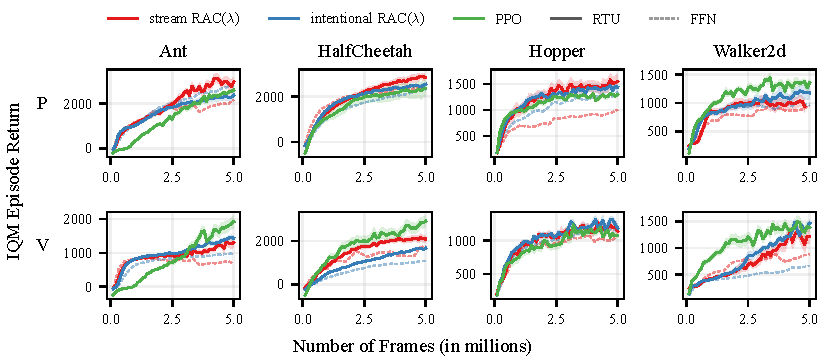
\includegraphics[width=\linewidth]{plots/mujoco/learning_curves.pdf}
    \caption{IQM episodic return with standard error, 10 seeds, on four MuJoCo tasks under masked velocities (\textbf{P}) and masked positions (\textbf{V}). Streaming methods use $\lambda = 0.99$, and \gls{ppo} uses the same network as the streaming agents (Appendix~\ref{sec:hyperparameters}). Solid curves use an \gls{rtu} recurrence, dashed curves the same algorithm with a feedforward network. Intentional RAC($\lambda$) uses the trace-estimated preconditioner and $\eta_\pi = 0.01$ (Appendix~\ref{sec:stepsize}).}
    \vspace{-0.3cm}
    \label{fig:brax}
\end{figure}

\paragraph{Memoryless control.}
The dashed curves are the same updates with the recurrence removed, at the same budget and seed
count. Bootstrapping that difference at 5M, the recurrence is ahead on six of eight cells for
stream RAC($\lambda$), from $+506$ to $+973$, and on four of eight for intentional RAC($\lambda$),
from $+314$ to $+774$. Neither is behind on any cell, so the recurrence earns its place under both
updates, and more reliably under the one whose step size transfers.

\paragraph{Result.}
Stream RAC($\lambda$) and recurrent \gls{ppo} are statistically indistinguishable on most of the
benchmark (Figure~\ref{fig:brax}). Bootstrapping the difference of means over the 10 seeds per cell separates only three of eight, with \gls{ppo} ahead on
Ant-V and Walker2d-P, stream RAC($\lambda$) on Hopper-V, and the other five overlap. Appendix~\ref{sec:stepsize} lists the
per-cell intervals. We therefore claim parity rather than an advantage.

Most of the difference from the setting these methods ship with is the trace decay, since at
$\lambda = 0.8$ stream RAC($\lambda$) reaches $262$ on Hopper-P against $1550$ at $0.99$, a
factor of $5.9$ (Appendix~\ref{sec:lambda}). Walker2d resisted $\lambda$, a per-block step size, removing the
entropy bonus and matching the network size, and responded only to the actor step size under the
intentional update (Appendix~\ref{sec:stepsize}).

Intentional RAC($\lambda$) does not complete the benchmark as published, since on three cells its
updates become non-finite partway through training.
Appendix~\ref{sec:stepsize-analysis} attributes this to its preconditioner and shows that
estimating it from the trace instead removes the divergence, after which all eight cells complete
on every seed. Its actor step size does not transfer either. At $\eta_\pi = 0.01$ rather than the
$0.05$ of \citet{sharifnassab2026intentional} it improves on seven of eight cells and reaches
parity with stream RAC($\lambda$), ahead on one cell, behind on two and indistinguishable on five,
and with recurrent \gls{ppo}, ahead on two, behind on two and indistinguishable on four.

\begin{figure}[t]
    \centering
    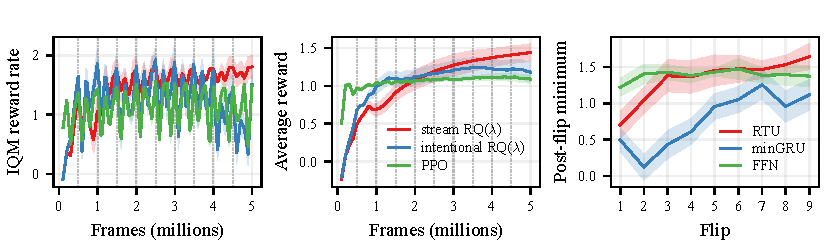
\includegraphics[width=\linewidth]{plots/foragax/foragax_body.pdf}
    \caption{Continual foraging, 10 seeds. Left and centre compare the algorithms under
    \gls{rtu}: the reward rate, an exponential moving average that tracks current performance,
    and the average reward over the agent's lifetime, the statistic of \citet{tang2026forager}.
    Right compares the recurrences within stream RQ($\lambda$), showing the minimum reward rate reached
    after each of the nine reward flips. Dotted lines mark the flips.}
    \label{fig:foragax}
\end{figure}

\subsection{Continual Foraging}
\label{sec:foragax}

A memoryless agent relearns after every flip, and the recurrent state takes the flips over.

\paragraph{Task and design.}
Foragax NeverEndingRelearning \citep{tang2026forager} is a grid world whose two biomes swap their mushroom rewards every 500k frames, so the agent must repeatedly abandon a learned foraging pattern and rediscover the other biome. Following \citet{tang2026forager}, the agent sees a $9 \times 9$ one-hot aperture, is never reset, and explores $\varepsilon$-greedily with a floor of $0.1$. We run stream RQ($\lambda$) and intentional RQ($\lambda$) with \gls{rtu}, minGRU and a memoryless network (FFN) under \gls{rtrl}, and recurrent \gls{ppo} with \gls{rtu} at its tuned entropy coefficient, for 5M frames and 10 seeds (Figure~\ref{fig:foragax-curves}). \citet{tang2026forager} evaluate by average reward over the agent's lifetime. We report both that and the exponential moving average of reward, which they also use, because the post-flip recoveries are what this section is about and a lifetime average integrates them away.




\paragraph{Result.}
The flips can be absorbed by relearning the weights or by carrying the phase in the state, and
the post-flip minima separate the two. Stream RQ($\lambda$) ends at a reward rate of $1.73$ with
\gls{rtu}, $1.63$ with the FFN and $1.47$ with minGRU, against \gls{ppo} at $1.16$, a gap
of $0.56$ $[0.08, 0.95]$. Under the lifetime average of \citet{tang2026forager} the ordering
holds but the margin is unresolved, $1.42$ against $1.10$ $[-0.05, 0.45]$. The memoryless agent dips to
between $1.2$ and $1.4$ at every flip and \gls{ppo} to
between $0.5$ and $0.8$, whereas the \gls{rtu} dip shrinks from $0.70$ at the
first flip to $1.64$ at the ninth (Figure~\ref{fig:foragax}), so the recurrent state progressively
takes over the phase the FFN must relearn. The recurrence buys a shallower recovery rather than a
higher ceiling, \gls{rtu} and the FFN finishing at $1.73$ and $1.63$. Which update it is paired
with matters more than the recurrence itself, since \gls{rtu} costs stream RQ($\lambda$) nothing,
$+0.05$ $[-0.42, 0.40]$, and intentional RQ($\lambda$) $-0.81$ $[-1.22, -0.40]$, an interaction
of $0.85$ $[0.25, 1.41]$. Under intentional RQ($\lambda$) the memoryless
agent is the best agent here (Appendix~\ref{sec:stepsize-analysis}).

\section{Related work}
\label{sec:related}

Streaming deep RL was made stable with feedforward networks by step-size bounds that cap the
change in the prediction \citep{elsayed2024streaming}, pathwise actor updates that avoid a
growing score function \citep{vasan2024deep}, and intentional updates that solve for the step
directly \citep{sharifnassab2026intentional}. We keep that machinery unchanged and add the
recurrent channel. Appendix~\ref{sec:stepsize-analysis} shows all three of those step-size rules
rest on an assumption the sensitivity trace violates. Exact \gls{rtrl}
\citep{williams1989learning} is quartic in the hidden size, and has been made affordable either
by approximating the influence matrix \citep{tallec2017unbiased, menick2021practical,
bellec2020solution} or by restricting the recurrence so the exact influence is cheap, through
diagonal complex cells \citep{orvieto2023resurrecting, zucchet2023online, elelimy2024real} or
element-wise gates \citep{irie2024exploring}. We take the second route and analyse what the
resulting trace does inside a TD($\lambda$) update, which \citet{lemmel2025rtrrl} do not.
Recurrence is the standard remedy for partial observability, and \citet{ni2022recurrent} give
the baseline comparison our masked-MuJoCo protocol follows. Our continual-foraging evaluation
sits in the tradition of tracking rather than converging \citep{sutton2007tracking}, where the
failure mode is loss of plasticity \citep{dohare2024loss}, which Foragax
\citep{tang2026forager} induces with a periodically flipping reward.

\section{Discussion and Conclusion}
\label{sec:discussion}

Exact \gls{rtrl} over a diagonal recurrence substitutes for the truncated gradient in any
streaming algorithm built on a per-step gradient and an eligibility trace, and the two traces
compose into a credit horizon we predict, measure and follow from prediction through control.
Acting on the part of that horizon the composition leaves short moves masked
continuous control from a clear loss to parity.

The streaming agents trail recurrent
\gls{ppo} on eight of eleven POPGym tasks, three of which no method beats its memoryless
counterpart. Both intentional variants diverge until their preconditioner is
corrected, and on Foragax the best agent under that update is memoryless. Retention is necessary but not sufficient, since the credit
horizon exceeds the solvable chain in every MemoryChain cell. Two limitations are structural, a
single recurrent layer and ten seeds.

%%%%%%%%%%%%%%%%%%%%%%%%%%%%%%%%%%%%%%%%%%%%%%%%%%%%%%%%%%%%%%%%
%% Appendices
%%%%%%%%%%%%%%%%%%%%%%%%%%%%%%%%%%%%%%%%%%%%%%%%%%%%%%%%%%%%%%%%

\newpage

\subsubsection*{Reproducibility statement}

Proposition~\ref{prop:composition} is stated in Section~\ref{sec:methodology} and proved in
Appendix~\ref{sec:composition-proof}, with the staleness bound it relies on derived in
Appendix~\ref{sec:staleness-proof}. Appendix~\ref{sec:pseudocode} gives pseudocode for the
recurrent streaming update and the architecture, and Appendix~\ref{sec:hyperparameters} lists
every hyperparameter, network size and per-task setting, including the values taken unchanged
from the works each algorithm comes from and the two we retuned. Every benchmark is public and
unmodified apart from the observation masking described in Section~\ref{sec:mujoco}. All results
report seed counts in their captions, and every interval quoted in the text is a $95\%$
bootstrap percentile interval over seeds with $20{,}000$ resamples. The implementation is an
open-source framework for memory-augmented reinforcement learning which we will release on
acceptance, withheld here to preserve anonymity.

\subsubsection*{Ethics statement}

This work studies credit assignment in reinforcement learning agents on simulated control and
memory benchmarks. It involves no human subjects, no personal or sensitive data, and no
deployment on physical systems. We see no direct pathway to harm beyond the general dual-use
considerations that apply to reinforcement learning methods, and we comply with the ICLR Code of
Ethics.

\subsubsection*{Use of large language models}

Large language models were used as a general-purpose assistive tool, for code and experiment
scaffolding, for aggregating and plotting results, and for editing prose. They were not used to
generate research ideas, to derive or check the proofs, or to produce any experimental result.
All claims, derivations and numbers in this paper were verified by the authors, who take full
responsibility for the content.

\bibliography{main}
\bibliographystyle{iclr2026_conference}

\appendix
\section{MemoryChain solve rates}
\label{sec:memory-chain-grids}

Figure~\ref{fig:memory_chain_lambda} reports the difference in solve rate between the two
gradient computations. Figures~\ref{fig:grid-qrc}, \ref{fig:grid-stream-q} and
\ref{fig:grid-intentional-q} give the underlying per-method rates for each of the three
streaming algorithms, together with the difference. A run counts as successful when its final
return exceeds $0.5$; outlined cells mark, in each column, the longest chain at which the
method still succeeds on a majority of seeds.

\begin{figure}[H]
    \centering
    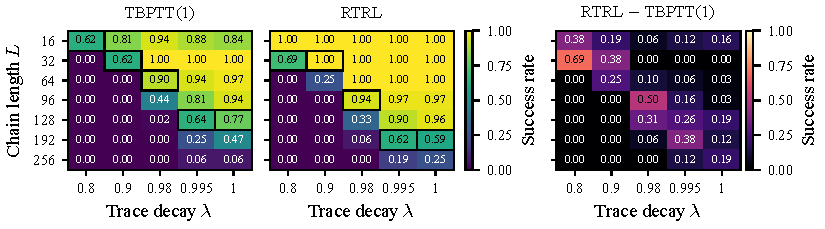
\includegraphics[width=\linewidth]{plots/memory_chain/horizon_grid.pdf}
    \caption{Solve rates for RQRC($\lambda$) with a minGRU recurrence ($\gamma{=}0.999$,
    $16$--$32$ seeds per cell). The solvable region under TBPTT(1) grows with the trace
    horizon, and exact \gls{rtrl} pushes that boundary one grid step deeper at every $\lambda$
    but $0.9$.}
    \label{fig:grid-qrc}
\end{figure}

\begin{figure}[H]
    \centering
    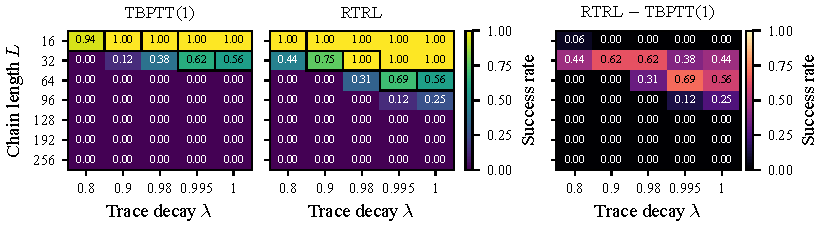
\includegraphics[width=\linewidth]{plots/memory_chain/horizon_grid_stream_q.pdf}
    \caption{Solve rates for stream RQ($\lambda$), which replaces RQRC($\lambda$)'s corrected
    update with \gls{obgd} on a single $Q$-network ($16$ seeds per cell). The qualitative
    structure is unchanged but the reachable horizon is roughly half as long, and past $L{=}32$
    TBPTT(1) fails at every $\lambda$ while \gls{rtrl} still solves a substantial fraction of
    seeds.}
    \label{fig:grid-stream-q}
\end{figure}

\begin{figure}[H]
    \centering
    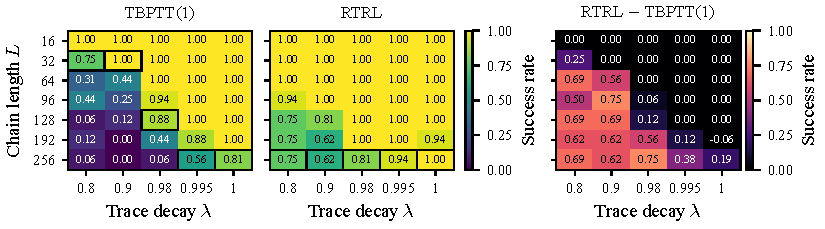
\includegraphics[width=\linewidth]{plots/memory_chain/horizon_grid_intentional_q.pdf}
    \caption{Solve rates for intentional RQ($\lambda$) ($16$ seeds per cell). Exact \gls{rtrl}
    solves a majority of seeds at every cell of the sweep, including $L{=}256$ at
    $\lambda{=}0.8$, so its reachable horizon is independent of $\lambda$ over this range,
    while TBPTT(1) still tracks the trace horizon.}
    \label{fig:grid-intentional-q}
\end{figure}

\section{Credit weight measurements in detail}

\subsection{Protocol and full measurements}
\label{sec:credit-appendix}

\paragraph{Task and design.}
Proposition~\ref{prop:composition} predicts the weight each update places on the immediate
Jacobian $\boldsymbol{I}_k$ of a step $n = T-k$ in the past, and \eqref{eq:amplification}
predicts how the two weights compare. Both are measurable. We train an agent with exact
\gls{rtrl} on MemoryChain with $L{=}64$ for $2 \times 10^5$ steps, freeze the parameters and
roll out episodes, for $10$ seeds per trace decay, cell and algorithm with $10$ rollouts per
seed. Because the recurrence is elementwise, both weights of Proposition~\ref{prop:composition}
assemble exactly from the recorded head gradients $\boldsymbol{c}_t$ and diagonal state Jacobians
$\boldsymbol{J}_t$ of a single rollout, and we fit the decay of $\|\boldsymbol{\omega}_k\|$ against
$n$ and compare it with the predicted rates at $\lambda{=}1$ and $\lambda{=}0.98$, the two
regimes of \eqref{eq:amplification}.

\paragraph{Result.}
Table~\ref{tab:weights} reports the measured rates. The TBPTT(1) weight decays at
$\gamma\lambda$ to within $0.2\%$ in every row, and the \gls{rtrl} weight at
$\max(\gamma\lambda,\rho)$ to within $2\%$, for both cells and both trace decays, confirming
Proposition~\ref{prop:composition} directly. Repeating the measurement under stream
$Q(\lambda)$ and intentional RQ($\lambda$) gives the same agreement, so the decomposition holds
across all three algorithms of Section~\ref{sec:memory_chain}.

Three further facts come out of the same measurements, detailed in
Appendix~\ref{sec:credit-appendix}. The amplification is cell-dependent, $20$ to $33$ at
$n{=}32$ for minGRU against $6$ to $9$ for \gls{rtu}, and the cause is phase cancellation:
minGRU's coherence $\|\sum_i \boldsymbol{t}_i\| / \sum_i \|\boldsymbol{t}_i\|$ is exactly $1$ at
every lag because its retentions are real and positive, while \gls{rtu}'s complex rotation
drives it to $0.23$--$0.46$ by $n{=}32$. Retention is learned for minGRU, which begins at
$\rho{=}0.5$ and reaches $0.981$ to $0.99995$ depending on the algorithm, and initialised for
\gls{rtu}, which begins at $0.997$. And exploration cuts favour \gls{rtrl}: both implementations
zero the eligibility trace on a non-greedy action but leave $\boldsymbol{S}_t$ intact, so a cut
deletes every TBPTT(1) weight before it while the \gls{rtrl} weight survives through the
influence matrix, which on trained minGRU agents leaves TBPTT(1) with no credit at $n{=}32$ in
$0.67$ to $0.77$ of rollouts at $\epsilon{=}0.1$. What the measurements do not establish is
sufficiency: the credit horizon exceeds the observed solvable chain in every cell of every grid.





This appendix records the full per-lag measurements behind Table~\ref{tab:weights} and the
discussion of Section~\ref{sec:weights}.

\paragraph{Ratio growth and regimes.}
Table~\ref{tab:weights} reports the measured rates. The decay of
$\boldsymbol{\omega}_k^{\mathrm{TBPTT(1)}}$ matches $\gamma\lambda$ at both trace
decays, with the predicted value falling inside the interquartile range in each
case, consistent with the first weight of Proposition~\ref{prop:composition}.
The measured $\rho$ is $0.999$ at both settings and is left unchanged by
$\lambda$, which is what the second weight requires. The gated units that carry
the cue saturate towards perfect retention, so lowering $\lambda$ moves
$\gamma\lambda$ away from one while leaving $\rho$ where it is, and only the
TBPTT(1) channel degrades. The weight under exact \gls{rtrl} correspondingly
decays at a rate close to one in both cases, within $1.5\%$ of
$\max(\gamma\lambda,\rho)$ at $\lambda{=}1$ and within $0.6\%$ at
$\lambda{=}0.98$.

The ratio of the two weights grows with the lag, reaching a median of $20$ at
$n{=}32$ for $\lambda{=}1$ and $33$ for $\lambda{=}0.98$. This growth is roughly
linear in $n$ at both settings rather than separating into the two regimes of
\eqref{eq:amplification}: at $\lambda{=}0.98$ the exponential form
$(\rho/\gamma\lambda)^{n}$ evaluates to under $2$ at $n{=}32$, far below what we
measure, because the sum defining $\boldsymbol{\omega}_k^{\mathrm{\gls{rtrl}}}$
accumulates on the order of $n$ terms in either regime. The ratio is also the
noisiest quantity we measure, spanning an order of magnitude across seeds, so we
draw no regime distinction from it. What is robust is its size: exact \gls{rtrl}
assigns between one and one and a half orders of magnitude more credit to
parameter uses several tens of steps in the past, which is the quantity that the
solve rates in Section~\ref{sec:memory_chain} reflect.

\paragraph{Exploration cuts.}
The eligibility trace is zeroed on every non-greedy action and at episode boundaries, while
the \gls{rtrl} influence matrix is carried through unchanged. Writing $m$ for the last cut
at or before $T$, TBPTT(1) has $\boldsymbol{\omega}_k = 0$ for every $k \leq m$, whereas
$\boldsymbol{\omega}_j^{\mathrm{\gls{rtrl}}} = \sum_{i=\max(j,m+1)}^{T} (\gamma\lambda)^{T-i}
\boldsymbol{c}_i^\top \boldsymbol{\Phi}_{i,j}$ remains non-zero for $j \leq m$. We measure the
fraction of rollouts in which the TBPTT(1) weight at lag $n$ is exactly zero while the
\gls{rtrl} weight is not, on trained minGRU agents at $L{=}64$, ten seeds and three rollouts
per seed per $\epsilon$.

\begin{table}[H]
\centering
\begin{tabular}{llcccccc}
\toprule
Algorithm & $\lambda$ & $\epsilon$ & $n{=}4$ & $n{=}8$ & $n{=}16$ & $n{=}32$ \\
\midrule
stream RQ($\lambda$) & $1$ & $0.01$ & $0.00$ & $0.00$ & $0.07$ & $0.13$ \\
stream RQ($\lambda$) & $1$ & $0.1$ & $0.23$ & $0.27$ & $0.50$ & $0.67$ \\
stream RQ($\lambda$) & $0.98$ & $0.01$ & $0.03$ & $0.03$ & $0.03$ & $0.07$ \\
stream RQ($\lambda$) & $0.98$ & $0.1$ & $0.17$ & $0.23$ & $0.57$ & $0.77$ \\
RQRC($\lambda$) & $1$ & $0.01$ & $0.03$ & $0.03$ & $0.10$ & $0.20$ \\
RQRC($\lambda$) & $1$ & $0.1$ & $0.23$ & $0.27$ & $0.53$ & $0.73$ \\
\bottomrule
\end{tabular}
\caption{Fraction of rollouts in which a Watkins cut leaves TBPTT(1) with no credit at lag
$n$ while exact \gls{rtrl} retains some, on minGRU at $L{=}64$.}
\label{tab:watkins}
\end{table}

\section{Additional MemoryChain results}
\label{sec:memory-chain-extra}

\begin{figure}[H]
    \centering
    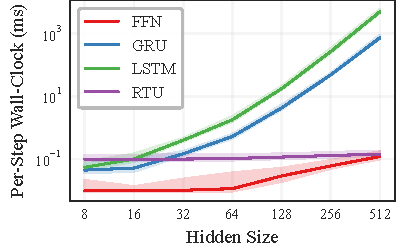
\includegraphics[width=0.52\linewidth]{plots/rtrl.pdf}
    \caption{Per-step wall-clock time (ms) of a single gradient update as a function of hidden
    width, comparing feedforward backpropagation (FFN) against exact \gls{rtrl} for \gls{gru},
    LSTM, and \gls{rtu} recurrent layers.}
    \label{fig:rtrl}
\end{figure}

\section{Additional Foragax results}
\label{sec:foragax-extra}

\begin{figure}[H]
    \centering
    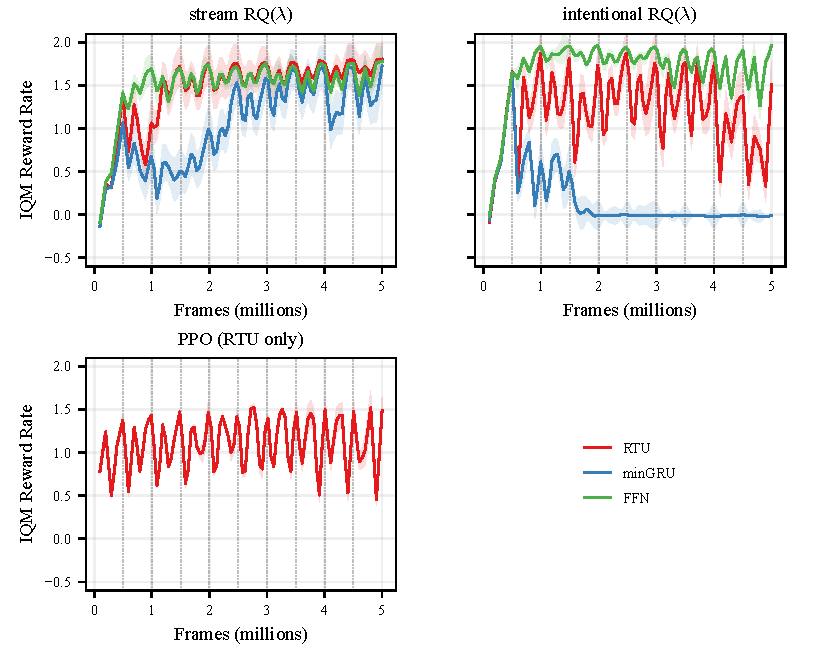
\includegraphics[width=\linewidth]{plots/foragax/reward_rate.pdf}
    \caption{IQM reward rate, 10 seeds, on Foragax NeverEndingRelearning for stream RQ($\lambda$), intentional RQ($\lambda$) and batched \gls{ppo} (entropy coefficient $0.1$), with the minimum after each flip in the last panel (solid stream RQ($\lambda$), dashed \gls{ppo}). Dotted lines mark the reward flips every 500k frames.}
    \label{fig:foragax-curves}
\end{figure}

\section{Step-size rules under a sensitivity trace}
\label{sec:stepsize-analysis}

Every streaming method here sets its step size from a norm of the eligibility trace. That is
sound when the trace is a decayed sum of recent gradients, because any coordinate carrying
trace mass has recently carried gradient mass. Exact \gls{rtrl} breaks the assumption: the
sensitivity gives a coordinate trace mass on steps where its instantaneous gradient is
negligible. We find the same assumption failing in three different rules.

\paragraph{\gls{obgd} bounds overshoot with an $\ell_1$ norm.} Its step is
$\alpha/\max(1, \bar{\delta}\|z\|_1 \alpha \kappa)$ with $\bar{\delta} = \max(|\delta|, 1)$,
which normalised rewards pin at exactly $1$, so the step is set purely by $\|z\|_1$. Under
\gls{rtrl} the trace is dense and that norm grows through training: on masked Hopper the
actor's $\|z\|_1$ rises from $4.5\times10^3$ to $1.35\times10^4$ and its step falls from
$8.9\times10^{-5}$ to $3.2\times10^{-5}$, while the critic, whose trace stays flat, is
unaffected. The mass is also badly distributed: measured on the masked-Hopper actor, the
\gls{rtu} block holds $91\%$ of the parameters and $19\%$ of the $\ell_1$ gradient mass, while
the policy head holds $2\%$ of the parameters and $74\%$ of the mass, so one small block sets
the step for the whole network. Sweeping $\kappa$ and $\eta$ does not repair this
(Appendix~\ref{sec:stepsize}), and neither does replacing the $\ell_1$ norm with a per-block
bound, which is worse on three of four cells at 5M.

\paragraph{Scale-free rules walk the retention.} Adam takes a step of order its learning rate
per parameter regardless of gradient magnitude, so it moves the recurrence's retention
parameter whether or not that gradient is informative. Training a pathwise actor-critic this
way on masked HalfCheetah drives \gls{rtu}'s $\rho$ from $0.99949$ to $0.99953$; the
steady-state gain $1/(1-\rho)$ passes $2000$, the cell integrates a drifting observation for a
thousand uninterrupted steps, and the carry overflows. Gradient clipping does not help, since
Adam renormalises immediately after the clip.

\paragraph{Preconditioners estimated on the wrong quantity.} The intentional update forms a
per-parameter second moment from the gradient, $m = \sqrt{\hat{v}} + \epsilon$ with
$v \leftarrow \beta_2 v + (1-\beta_2) g^2$, and then divides the trace by it, both in its
denominator $\sqrt{\hat{\sigma}\sum z^2/m}$ and in the update direction $z/m$. When the
sensitivity puts mass into coordinates the gradient rarely visits, $v$ stays near zero for
those coordinates while $z$ does not, and $z^2/m$ is inflated by a preconditioner that never
saw them. The symptoms follow: on masked Hopper the actor step is sixteen times smaller than
stream RAC($\lambda$)'s at the same $\lambda$, and on three MuJoCo cells and on Foragax the
updates become non-finite outright.

\paragraph{Trace preconditioning.} The fix is to estimate the second moment from the trace,
$v \leftarrow \beta_2 v + (1-\beta_2) z^2$, so the preconditioner covers what it divides.
Figure~\ref{fig:precondition} shows the effect on Foragax, where intentional RQ($\lambda$)
with \gls{rtu} is otherwise dead from $700$k frames onward: it recovers to a reward rate of
about $1.7$. The change also helps the memoryless agent, from $1.6$ to $1.9$, which says the
mismatch is not purely an \gls{rtrl} effect. An eligibility trace at $\lambda = 0.8$ already
accumulates mass in rarely visited coordinates, and the sensitivity makes an existing problem
acute. On masked MuJoCo the same change removes the divergence outright: intentional RAC($\lambda$)
completes all eight cells on all ten seeds where three previously failed, and improves on seven
of them.

It is not, however, a better preconditioner in general, and we would discourage adopting it as
one. Where the original is stable it costs performance: on six POPGym tasks it is worse on every
one, RepeatPrevious falling from $0.99$ to $0.68$, CountRecall from $-0.53$ to $-0.96$ and
Battleship from $-0.27$ to $-1.21$. On Foragax it is also a mitigation rather than a cure, since
the \gls{rtu} run still becomes non-finite late in training and minGRU recovers only to about
$0.3$. The pattern across the three benchmarks is that estimating the preconditioner from the
trace helps exactly where the gradient-estimated one diverges and hurts where it does not.

\begin{figure}[H]
    \centering
    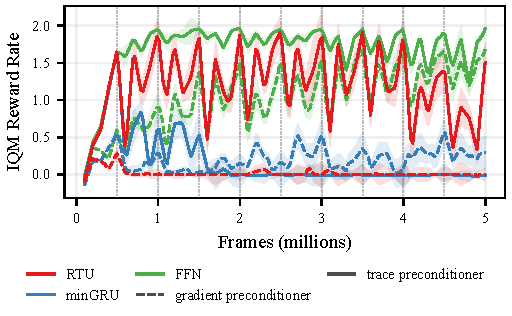
\includegraphics[width=0.62\linewidth]{plots/foragax/trace_preconditioning.pdf}
    \caption{Intentional RQ($\lambda$) on Foragax with the preconditioner estimated from the
    trace (solid) and from the gradient (dashed), IQM over 10 seeds with standard error.}
    \label{fig:precondition}
\end{figure}

\section{Trace decay on masked MuJoCo}
\label{sec:lambda}

Proposition~\ref{prop:composition} gives the credit on a step $k$ in the past a weight that
decays at $\max(\gamma\lambda, \rho)$, and with \gls{rtu}'s initialisation $\rho \approx
0.997$, which invites reading $\lambda$ as irrelevant. That reading holds only for the
recurrent parameters. Their gradient carries the \gls{rtrl} sensitivity, so their credit is
a convolution of $(\gamma\lambda)^k$ and $\rho^k$ and the slower mode wins. The feature
extractor and the head have no sensitivity path, so their credit decays at
$(\gamma\lambda)^k$ alone: a horizon of $4.8$ steps at $\lambda = 0.8$ against the
recurrence's $333$. The composition therefore buys a long horizon for the recurrence and
leaves the rest of the network short, and on a masked task the rest of the network is what
has to learn what the inferred state is worth.

Table~\ref{tab:lambda} sweeps $\lambda$ on masked Hopper at 2M frames with 5 seeds. That
cell was chosen because it had the largest gap to recurrent \gls{ppo} under the $\lambda = 0.8$
configuration. At $\lambda = 0.99$ it becomes a win, so the selection was made under the
setting the sweep then changed. Performance rises by a factor of $5.6$ between $\lambda = 0.8$
and $\lambda = 0.99$ and falls again at $\lambda = 1$. The corresponding factor in the main
experiment, at 5M frames with 10 seeds, is $5.9$.

The composition explains why $\lambda$ matters here at all, and does not predict where the
optimum falls. It says the parameters the sensitivity reaches inherit $\rho$ while the rest of
the network decays at $\gamma\lambda$, so on a task whose difficulty is state inference the
non-recurrent parameters are the binding constraint and lengthening their horizon should help;
it does. It does not say the horizon should be lengthened without limit, and the data show it
should not: $\lambda = 1$ brings $\gamma\lambda$ closer to $\rho$ than $\lambda = 0.99$ does
and performs worse, and the optimum sits at a horizon of $50$ against a retention horizon of
roughly $333$. That turn is the ordinary bias-variance trade-off of TD($\lambda$), with an
undecayed trace paying in variance what it gains in bias, and we report it as such rather than
as a prediction of Proposition~\ref{prop:composition}.

We use $\lambda = 0.99$ for masked MuJoCo throughout. Both source papers use $0.8$, which was
selected on fully observed control where no part of the network has to integrate an
observation stream. We did not sweep \gls{ppo}'s GAE $\lambda$, which stays at the $0.95$ of
\citet{elelimy2024real}; a reader should weigh the comparison accordingly.

The value does not transfer. Sweeping the same three settings elsewhere places the optimum in a
different place on every benchmark. On trace conditioning with \gls{rtu}, the return error at
ISI 20 is $0.036$ at $\lambda = 0.9$, $0.032$ at $0.95$ and $0.045$ at $0.99$, and at ISI 40
$0.090$, $0.059$ and $0.064$, so $0.95$ is best and $0.99$ is worse. On POPGym the direction is algorithm-dependent. Raising
$\lambda$ to $0.99$ from the value each method reports takes stream RQ($\lambda$) on
RepeatPrevious from $0.05$ to $0.93$ in raw return, while it takes intentional RQ($\lambda$) on
the same task from $0.83$ to $-0.12$ and leaves RQRC($\lambda$) near its $0.95$ value. What generalises is that an interior optimum exists and that it sits
far below the retention horizon. Where it sits does not, and we report $\lambda$ as a
benchmark-level choice rather than a quantity the composition determines.

\begin{table}[H]
\centering
\caption{Episode return at 2M frames on masked Hopper against the trace decay, mean over 5
seeds with standard error, stream RAC($\lambda$) with \gls{rtu} under exact \gls{rtrl}.}
\label{tab:lambda}
\begin{tabular}{lrrr}
\toprule
$\lambda$ & $\gamma\lambda$ & horizon $1/(1-\gamma\lambda)$ & return \\
\midrule
$0.8$  & $0.792$ & $4.8$   & $223 \pm 7$ \\
$0.95$ & $0.940$ & $16.8$  & $1041 \pm 71$ \\
$0.99$ & $0.980$ & $50.3$  & $\mathbf{1255 \pm 51}$ \\
$1.0$  & $0.990$ & $100.0$ & $1089 \pm 119$ \\
\bottomrule
\end{tabular}
\end{table}

Lengthening the trace also changes what every streaming step-size rule does, because each
normalises by a norm of that trace. \gls{obgd} bounds overshoot by $\bar{\delta}\|z\|_1$, so
a longer trace shrinks its step roughly in proportion and the product of step and trace stays
stable. The intentional update divides by $\sqrt{\sigma \|z\|^2}$ where $\sigma$ itself grows
with the trace, so it pays for the extra length twice: on masked Hopper its actor step falls
from $5.5\times10^{-6}$ at $\lambda=0.8$ to $8.4\times10^{-7}$ at $\lambda=0.99$, sixteen
times smaller than stream RAC($\lambda$) on the same task, and it recovers far less of the
gap. Raising $\lambda$ without revisiting the step-size constant is therefore not a safe
default.

\section{Actor step-size sweep on masked MuJoCo}
\label{sec:stepsize}

\begin{table}[H]
\centering
\caption{Masked MuJoCo at 5M frames, 10 seeds. Bootstrap $95\%$ percentile interval on the
difference of means, stream RAC($\lambda$) minus recurrent \gls{ppo}, from $20{,}000$ resamples.
An interval excluding zero separates the two methods.}
\label{tab:mujoco-intervals}
\begin{tabular}{lrrrr}
\toprule
Cell & stream RAC($\lambda$) & \gls{ppo} & Difference & $95\%$ interval \\
\midrule
Ant-P         & $2944$ & $2605$ & $+339$ & $[-74, 747]$ \\
Ant-V         & $1437$ & $1936$ & $-499$ & $[-926, -63]$ \\
HalfCheetah-P & $2928$ & $2449$ & $+479$ & $[-237, 1182]$ \\
HalfCheetah-V & $2146$ & $2742$ & $-596$ & $[-1180, 14]$ \\
Hopper-P      & $1550$ & $1312$ & $+238$ & $[-34, 513]$ \\
Hopper-V      & $1214$ & $1082$ & $+132$ & $[1, 287]$ \\
Walker2d-P    & $1073$ & $1386$ & $-313$ & $[-557, -27]$ \\
Walker2d-V    & $1207$ & $1330$ & $-123$ & $[-426, 190]$ \\
\bottomrule
\end{tabular}
\end{table}


Under \gls{obgd} the effective actor step is $\alpha / \max(1, \alpha \kappa_\pi
\bar{\delta} \|z\|_1)$, and with a Gaussian policy the score function grows as the policy
sharpens, so $\|z\|_1$ grows and the step falls over training. Table~\ref{tab:stepsize} sweeps
the actor constant of both methods in both directions on the two cells where the gap to recurrent
\gls{ppo} is widest, at 2M frames with 10 seeds and $\lambda = 0.99$, holding each critic
constant at its default. The two methods behave differently. Stream RAC($\lambda$) peaks at the
$\kappa_\pi = 3$ it ships with and falls away on both sides, so its constant transfers to this
setting. Intentional RAC($\lambda$) does not: it peaks at $\eta_\pi = 0.01$, five times smaller
than the published $0.05$, gaining $+429$ on Hopper-P and $+450$ on Walker2d-P, while every
increase above the default is worse. Section~\ref{sec:mujoco} reports it at the corrected value.
The same argument that sets $\lambda$ for the recurrence rather than inheriting it applies to the
step size, and only one of the two published constants survives it.

\begin{table}[H]
\centering
\caption{Final episode return at 2M frames on masked MuJoCo under actor step-size sweeps at
$\lambda = 0.99$, mean over 10 seeds with standard error. Each method is bracketed on both sides
of the constant its source paper uses.}
\label{tab:stepsize}
\begin{tabular}{llrr}
\toprule
Method & Actor constant & Hopper-P & Walker2d-P \\
\midrule
stream RAC($\lambda$)      & $\kappa_\pi = 0.3$          & $176 \pm 70$   & $170 \pm 42$ \\
                           & $\kappa_\pi = 1$            & $921 \pm 167$  & $717 \pm 77$ \\
                           & $\kappa_\pi = 3$ (published) & $\mathbf{1259 \pm 62}$ & $\mathbf{925 \pm 45}$ \\
                           & $\kappa_\pi = 6$            & $1005 \pm 59$  & $715 \pm 76$ \\
                           & $\kappa_\pi = 10$           & $809 \pm 68$   & $642 \pm 88$ \\
\midrule
intentional RAC($\lambda$) & $\eta_\pi = 0.005$          & $1003 \pm 58$  & $1001 \pm 40$ \\
                           & $\eta_\pi = 0.01$           & $\mathbf{1296 \pm 78}$ & $\mathbf{1011 \pm 47}$ \\
                           & $\eta_\pi = 0.05$ (published) & $867 \pm 50$ & $561 \pm 40$ \\
                           & $\eta_\pi = 0.2$            & $324 \pm 63$   & $263 \pm 44$ \\
                           & $\eta_\pi = 1$              & $168 \pm 34$   & $183 \pm 38$ \\
\midrule
recurrent \gls{ppo}        & ---                         & $1121 \pm 50$  & $1164 \pm 49$ \\
\bottomrule
\end{tabular}
\end{table}

\section{POPGym with other recurrences}
\label{sec:popgym-cells}

The recurrence is not held constant across benchmarks, since MemoryChain uses minGRU, POPGym and
masked MuJoCo use \gls{rtu}, and trace conditioning reports both. MemoryChain uses minGRU because
it reaches longer chains there, and the two cells order differently on the other benchmarks,
since \gls{rtu} leads minGRU at every interstimulus interval but $80$ in
Section~\ref{sec:trace}. Figures~\ref{fig:popgym-mingru}
and~\ref{fig:popgym-ffn} therefore repeat the POPGym sweep with a minGRU recurrence and with a
memoryless network, at the same budget and seed count as the \gls{rtu} figure in
Section~\ref{sec:popgym}. The ordering among algorithms is largely preserved, but the cell matters where the
task rewards accumulation: on MultiArmedBandit a minGRU under stream RQ($\lambda$) reaches $0.76$
against $0.55$ for \gls{rtu}, a gap of $+0.21$ $[+0.20, +0.22]$, and beats its own memoryless
control by $+0.13$ where \gls{rtu} falls $0.08$ below it. Estimating the value of an arm is a
running average, which real positive retentions accumulate coherently and a complex rotation does
not, the same phase cancellation Section~\ref{sec:weights} measures. The memoryless comparison is
what the per-task ceilings in Section~\ref{sec:popgym} are computed from. Foragax reports the same
three recurrences in Section~\ref{sec:foragax}. We did not run masked MuJoCo with a second
recurrence, so the cell and the benchmark remain confounded there alone.

\begin{figure}[H]
    \centering
    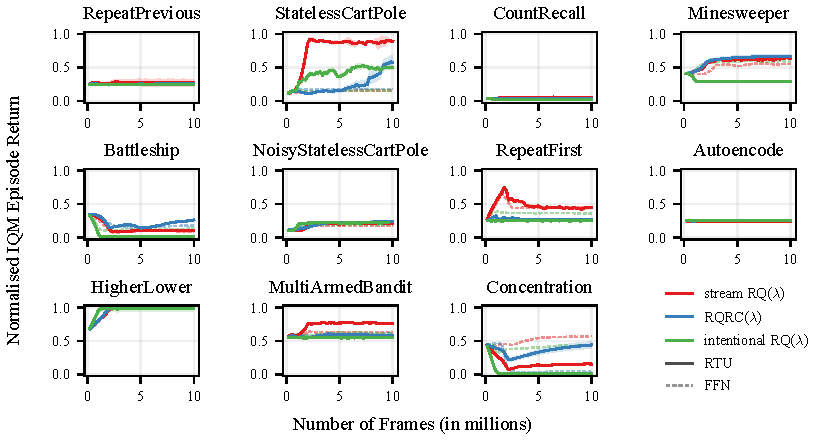
\includegraphics[width=\linewidth]{plots/popgym/learning_curves_mingru.pdf}
    \caption{POPGym with a minGRU recurrence, otherwise identical to
    Figure~\ref{fig:popgym}. Normalised IQM episodic return over 10 seeds with standard error,
    with dashed curves giving the same algorithms with a feedforward network.}
    \label{fig:popgym-mingru}
\end{figure}

\begin{figure}[H]
    \centering
    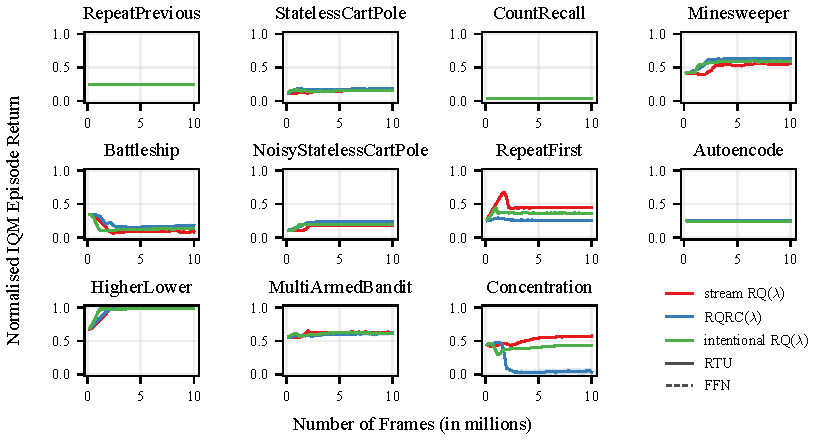
\includegraphics[width=\linewidth]{plots/popgym/learning_curves_ffn.pdf}
    \caption{POPGym with a memoryless network, otherwise identical to
    Figure~\ref{fig:popgym}. These runs are what the per-task memoryless ceilings of
    Section~\ref{sec:popgym} are estimated from on the two cartpole variants.}
    \label{fig:popgym-ffn}
\end{figure}

\section{Frozen-recurrence control}
\label{sec:frozen-control}

Table~\ref{tab:frozen} reports the frozen-recurrence control referred to in
Section~\ref{sec:memory_chain}: RQRC($\lambda$) with TBPTT(1) on a cell whose recurrent
parameters stay at initialisation. A random \gls{rtu} with $\rho \approx 0.997$ and the
eligibility trace solve $L{=}16$ in about half the seeds and nothing beyond $L{=}32$, and a
frozen minGRU solves nothing, so the trained recurrence is required and a long-retention
reservoir does not substitute for it.

\begin{table}[H]
\centering
\caption{Mean MemoryChain score with the recurrent parameters frozen at initialisation, RQRC($\lambda$) with TBPTT(1), 16 seeds.}
\label{tab:frozen}
\begin{tabular}{llccccccc}
\toprule
Cell & $\lambda$ & $L{=}16$ & $32$ & $64$ & $96$ & $128$ & $192$ & $256$ \\
\midrule
\gls{rtu} & $0.95$ & $0.57$ & $0.15$ & -- & $0.05$ & $0.00$ & $0.02$ & $-0.02$ \\
\gls{rtu} & $1$ & $0.55$ & $0.27$ & $0.01$ & $0.02$ & $0.01$ & $-0.02$ & $0.02$ \\
minGRU & $0.95$ & $0.08$ & $0.02$ & $0.01$ & $-0.03$ & $0.01$ & $-0.06$ & $-0.01$ \\
minGRU & $1$ & $-0.02$ & $-0.01$ & $-0.01$ & $0.01$ & -- & $-0.03$ & $0.04$ \\
\bottomrule
\end{tabular}
\end{table}

\section{Hyperparameters}
  \label{sec:hyperparameters}

We used fully connected networks of width $64$ with a single hidden block for MemoryChain and POPGym, and of width $128$ with two hidden blocks for Masked MuJoCo, following \citet{sharifnassab2026intentional}. All use LeakyReLU activations with LayerNorm \citep{ba2016layer} before each activation. On masked MuJoCo the \gls{ppo} baseline is given the same body as the streaming agents, two width-$128$ blocks with LayerNorm, LeakyReLU and the same $90\%$ sparse initialisation, and no projection after the recurrence, so that the comparison is at matched capacity: $139{,}405$ parameters against $141{,}709$, the difference being the streaming actor's state-dependent standard deviation head. It keeps its own orthogonal head initialisations, which are a stability device rather than a capacity choice. On MemoryChain and POPGym it keeps its standard width-$64$ $\tanh$ network with orthogonal initialisation. A single \gls{rtu}
layer of hidden dimension $192$ is inserted between the input and
output blocks. We used separate networks for the policy and value
functions. For stream RAC($\lambda$) we used softmax policy parameterization in
discrete control and a Gaussian with state-dependent standard deviation and actions clipped to $[-1, 1]$ in continuous control. For RQRC($\lambda$) we used an
$\varepsilon$-greedy policy. We used sparse
initialization with a sparsity ratio of $90\%$
\citep{elsayed2024streaming} and normalized observations and rewards
online with running statistics. stream RAC($\lambda$) uses ObGD with step size
$\alpha = 1$; the per-benchmark $\kappa$ values for the policy and
value networks are listed in the experiment-specific tables below. RQRC($\lambda$)
uses SGD with global-norm gradient clipping at $1.0$ and learning rates
$10^{-4}$ for the Q-network and $10^{-5}$ for the auxiliary
$h$-network. For the \gls{ppo} baseline we used the
hyperparameters reported by \citet{elelimy2024real}, including their real-time update:
a rollout of $2048$ steps, each stored with its own \gls{rtrl} sensitivity, split into
$32$ minibatches of single steps.

\begin{table}[H]
\centering
\caption{Hyperparameters for RQRC($\lambda$) on the MemoryChain experiment
(Section~\ref{sec:memory_chain}).}
\label{tab:hparams-MemoryChain}
\begin{tabular}{ll}
\toprule
Name & Value \\
\midrule
Chain length, $L$                      & $\{2, 4, 8, 16, 32, 48, 64, 128\}$ \\
Frames per run                         & $500{,}000$ \\
Number of seeds                        & $16$--$32$ per cell \\
Discount factor, $\gamma$              & $0.999$ \\
Trace decay, $\lambda$                 & $0.95$ \\
$Q$-network step size, $\alpha_Q$      & $10^{-4}$ \\
$h$-network step size, $\alpha_h$      & $10^{-5}$ \\
Regularization coefficient, $\beta$ & $1.0$ \\
MLP width                              & $64$ \\
\gls{rtu} hidden dimension             & $192$ \\
\bottomrule
\end{tabular}
\end{table}

\begin{table}[H]
\centering
\caption{Hyperparameters for RQRC($\lambda$) on POPGym (Section~\ref{sec:popgym}).}
\label{tab:hparams-popgym-streaming}
\begin{tabular}{ll}
\toprule
Name & Value \\
\midrule
Frames per run                         & $10{,}000{,}000$ \\
Number of seeds                        & $10$ \\
Discount factor, $\gamma$              & $0.99$ \\
Trace decay, $\lambda$                 & $0.95$ \\
$Q$-network step size, $\alpha_Q$      & $10^{-4}$ \\
$h$-network step size, $\alpha_h$      & $10^{-5}$ \\
Regularization coefficient, $\beta$ & $1.0$ \\
$\varepsilon$ schedule             & $1.0 \to 0.01$ over $20\%$ of training \\
MLP width                              & $64$ \\
\gls{rtu} hidden dimension             & $192$ \\
\bottomrule
\end{tabular}
\end{table}



\begin{table}[H]
\centering
\caption{Hyperparameters for the Masked MuJoCo experiment
(Section~\ref{sec:mujoco}). Stream RAC($\lambda$) and intentional RAC($\lambda$)
share the network, discount and trace decay and differ only in the optimizer.}
\label{tab:hparams-mujoco}
\begin{tabular}{ll}
\toprule
Name & Value \\
\midrule
Frames per run                         & $5{,}000{,}000$ \\
Number of seeds                        & $10$ \\
Observation regimes                    & masked velocities (\textbf{P}), masked positions (\textbf{V}) \\
Discount factor, $\gamma$              & $0.99$ \\
Trace decay, $\lambda$                 & $0.99$ (see Appendix~\ref{sec:lambda}) \\
Entropy coefficient                    & $0.01$ \\
MLP width (two blocks)                 & $128$ \\
\gls{rtu} hidden dimension             & $192$ \\
\midrule
Stream RAC($\lambda$) optimizer        & ObGD \\
Actor step size, $\alpha_\pi$          & $1.0$ \\
Critic step size, $\alpha_V$           & $1.0$ \\
Actor $\kappa_\pi$                     & $3.0$ \\
Critic $\kappa_V$                      & $2.0$ \\
\midrule
Intentional RAC($\lambda$) optimizer   & intentional update, trace-estimated preconditioner \\
Actor $\eta_\pi$                       & $0.01$ (see Appendix~\ref{sec:stepsize}) \\
Critic $\eta_V$                        & $0.5$ \\
\midrule
\gls{ppo} network                      & matched to the streaming agents (see above) \\
\gls{ppo} rollout length               & $2048$ \\
\gls{ppo} single-step minibatches, epochs & $32$, $4$ \\
\gls{ppo} GAE $\lambda$                & $0.95$ \\
\gls{ppo} clip coefficient             & $0.2$ \\
\gls{ppo} entropy coefficient          & $0.0$ \\
\gls{ppo} step size (Adam), grad clip  & $10^{-4}$, $0.5$ \\
\bottomrule
\end{tabular}
\end{table}

\begin{table}[H]
\centering
\caption{Hyperparameters for the trace-conditioning experiment (Section~\ref{sec:trace}), following \citet{rafiee2022eye}.}
\label{tab:hparams-trace}
\begin{tabular}{ll}
\toprule
Name & Value \\
\midrule
Steps per run                          & $2{,}000{,}000$ \\
Number of seeds                        & $10$ \\
Nominal ISI and discount $\gamma$      & $10$: $0.9$, $20$: $0.95$, $40$: $0.975$, $80$: $0.9875$ \\
ISI range                              & $[\mathrm{ISI} - \lfloor \mathrm{ISI}/3 \rfloor, \mathrm{ISI} + \lfloor \mathrm{ISI}/3 \rfloor]$ \\
Inter-trial interval                   & $[80, 120]$ steps \\
Activation lengths (CS, US)            & $4$, $2$ steps \\
Trace decay, $\lambda$                 & $\{0.9, 1\}$ \\
Return-error horizon                   & $400$ steps \\
Optimizer                              & ObGD, $\alpha = 1$, $\kappa = 2$ \\
MLP width                              & $64$ \\
Recurrent hidden dimension             & $192$ \\
\bottomrule
\end{tabular}
\end{table}

\begin{table}[H]
\centering
\caption{Hyperparameters for the Foragax NeverEndingRelearning experiment
(Section~\ref{sec:foragax}). Stream RQ($\lambda$) and intentional RQ($\lambda$)
share the network, discount, trace decay and exploration schedule and differ
only in the optimizer.}
\label{tab:hparams-foragax}
\begin{tabular}{ll}
\toprule
Name & Value \\
\midrule
Frames per run                         & $5{,}000{,}000$ \\
Number of seeds                        & $10$ \\
Reward-flip period                     & $500{,}000$ frames \\
Observation                            & $9 \times 9$ aperture of one-hot object channels \\
Discount factor, $\gamma$              & $0.99$ \\
Trace decay, $\lambda$                 & $0.8$ \\
Exploration, $\varepsilon$             & $1.0 \to 0.1$ linearly over the first $10\%$ of frames \\
Convolution                            & $16$ filters, $3 \times 3$, valid padding \\
MLP width                              & $128$ \\
Recurrent hidden dimension             & $192$ \\
Reward-rate smoothing                  & exponential average with $\beta = 10^{-4}$ \\
\midrule
Stream RQ($\lambda$) optimizer          & ObGD \\
Step size, $\alpha$                    & $1.0$ \\
$\kappa$                               & $1.0$ \\
\midrule
Intentional RQ($\lambda$) optimizer    & intentional update \\
$\eta$                                 & $0.1$ \\
\midrule
\gls{ppo} rollout length               & $2048$ \\
\gls{ppo} single-step minibatches, epochs & $32$, $4$ \\
\gls{ppo} GAE $\lambda$                & $0.95$ \\
\gls{ppo} entropy coefficient          & $0.1$, selected from $\{0.01, 0.1, 1\}$ \\
\gls{ppo} step size (Adam)             & $3 \times 10^{-4}$ actor, $3 \times 10^{-3}$ critic \\
\gls{ppo} gradient clip                & $0.5$ \\
\bottomrule
\end{tabular}
\end{table}

  \begin{table}[H]
  \centering
  \caption{Hyperparameters for stream RAC($\lambda$) on the KMemoryChain experiment
  (Appendix~\ref{sec:staleness}).}
  \label{tab:hparams-StreamAC-KMemoryChain}
  \begin{tabular}{ll}
  \toprule
  Name & Value \\
  \midrule
  Memory length, $K$                     & $\{4, 8, 16\}$ \\
  Frames per run                         & $300{,}000$ \\
  Number of seeds                        & $5$ \\
  Discount factor, $\gamma$              & $0.99$ \\
  Trace decay, $\lambda$                 & $0.95$ \\
  Actor step size, $\alpha_\pi$          & $1.0$ \\
  Critic step size, $\alpha_v$           & $1.0$ \\
  Actor ObGD $\kappa_\pi$                & $3$ \\
  Critic ObGD $\kappa_v$                 & $2.0$ \\
  Entropy coefficient                    & $0.01$ \\
  \gls{rtu} feature dimension            & $64$ \\
  \gls{rtu} hidden dimension             & $192$ \\
  \bottomrule
  \end{tabular}
  \end{table}

  \begin{table}[H]
  \centering
  \caption{Hyperparameters for RQRC($\lambda$) on the KMemoryChain experiment
  (Appendix~\ref{sec:staleness}).}
  \label{tab:hparams-QRC-KMemoryChain}
  \begin{tabular}{ll}
  \toprule
  Name & Value \\
  \midrule
  Memory length, $K$                     & $\{4, 8, 16\}$ \\
  Frames per run                         & $300{,}000$ \\
  Number of seeds                        & $5$ \\
  Discount factor, $\gamma$              & $0.99$ \\
  Trace decay, $\lambda$                 & $0.95$ \\
  $Q$-network step size, $\alpha_Q$      & $10^{-4}$ \\
  $h$-network step size, $\alpha_h$      & $10^{-5}$ \\
  Regularization coefficient, $\beta$    & $1.0$ \\
  $\epsilon$-greedy start                & $1.0$ \\
  $\epsilon$-greedy end                  & $0.01$ \\
  $\epsilon$-greedy decay fraction       & $0.1$ \\
  \gls{rtu} feature dimension            & $64$ \\
  \gls{rtu} hidden dimension             & $192$ \\
  \bottomrule
  \end{tabular}
  \end{table}



\section{Pseudocode}
\label{sec:pseudocode}

\begin{figure}[H]
    \centering
    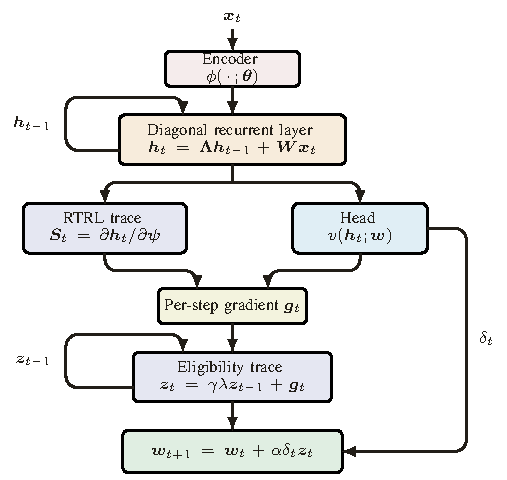
\includegraphics[width=0.62\linewidth]{figures/architecture.pdf}
    \caption{Data flow for one network with a value head. The recurrent layer's \gls{rtrl} trace and the head's gradient form $\boldsymbol{g}_t$, which the eligibility trace accumulates.}
    \label{fig:architecture}
\end{figure}


  The contribution to either parent algorithm is the per-step gradient
  computation: each network maintains an RTU hidden state $\boldsymbol{h}$ and a
  forward-mode RTRL sensitivity matrix $S = \partial \boldsymbol{h} / \partial \boldsymbol{\psi}$,
  both advanced once per environment step, and gradients of any scalar
  depending on $\boldsymbol{h}$ are computed from $S$. Following the
  parent algorithms, $\boldsymbol{\theta}$, $\boldsymbol{\psi}$ and $\boldsymbol{w}$ denote each network's full
  parameter set (encoder, RTU, head). Trace recursions and update rules are
  unchanged from the parents.

  \begin{algorithm}[H]
  \caption{RQRC($\lambda$) with RTU-RTRL}
  \label{alg:qrc_rtu}
  \begin{algorithmic}
    \State{Input: a differentiable action-value function parametrization $\hat{q}_{\boldsymbol{w}}$ with an RTU layer}
    \State{Input: a differentiable auxiliary function parametrization $\hat{h}_{\boldsymbol{\theta}}$ with an RTU layer}
    \State{Algorithm parameters: learning rate $\alpha_q$, $h$ learning rate $\alpha_h$, exploration parameter $\epsilon$.}
    \State{Initialize $\boldsymbol{z}_t^{\boldsymbol{\theta}} \leftarrow \boldsymbol{0}$}
    \State{Initialize $\boldsymbol{z}_t^{\boldsymbol{w}} \leftarrow \boldsymbol{0}$}
    \State{Initialize $z_t^h \leftarrow 0$}
    \State{Initialize RTU carries $\boldsymbol{h}_t^q, \boldsymbol{h}_t^h \leftarrow \boldsymbol{0}$ and RTRL traces $\boldsymbol{S}_t^q, \boldsymbol{S}_t^h \leftarrow \boldsymbol{0}$}
    \State{Observe initial state $\boldsymbol{S}_0$}
    \For{iteration $t = 1, 2, \cdots$}
      \State{Advance $(\boldsymbol{h}_t^q, \boldsymbol{S}_t^q)$ and $(\boldsymbol{h}_t^h, \boldsymbol{S}_t^h)$ one RTU step on $\boldsymbol{S}_t$.}
      \State{Sample an action $A_t \sim \pi$.} \Comment{We use an $\epsilon$-greedy policy.}
      \State{Take action $A_t$, observe $R_{t+1}$ and $S_{t+1}$.}
      \State{Compute $\delta_t$ and $\nabla_{\boldsymbol{w}_t} \delta_t$ as in RQRC($\lambda$) \citep{elelimy2025deep}, with parameter gradients of $\hat q_{\boldsymbol{w}}$ obtained from the
  RTRL trace $\boldsymbol{S}_t^q$.}
      \State{Update the traces $\boldsymbol{z}_t^{\boldsymbol{\theta}}$, $\boldsymbol{z}_t^{\boldsymbol{w}}$, and $z_t^h$ as in RQRC($\lambda$) \citep{elelimy2025deep}, with parameter
  gradients of $\hat h_{\boldsymbol{\theta}}$ obtained from the RTRL trace $\boldsymbol{S}_t^h$.}
      \State{Compute $\Delta \boldsymbol{w}_t$ and $\Delta \boldsymbol{\theta}_t$ as in RQRC($\lambda$) \citep{elelimy2025deep}.}
      \State{Update the parameters $\boldsymbol{w}_{t+1} \leftarrow \boldsymbol{w}_t + \alpha_q \Delta \boldsymbol{w}_t$.}
      \State{Update the parameters $\boldsymbol{\theta}_{t+1} \leftarrow \boldsymbol{\theta}_t + \alpha_h \Delta \boldsymbol{\theta}_t$.}
      \If{episode terminated or $A_t$ is non-greedy}
        \State{Reset the traces $\boldsymbol{z}_t^{\boldsymbol{\theta}}$, $\boldsymbol{z}_t^{\boldsymbol{w}}$, and $z_t^h$ to zeros.}
      \EndIf
      \If{episode terminated}
        \State{Reset the RTU carries $\boldsymbol{h}_t^q, \boldsymbol{h}_t^h$ and RTRL traces $\boldsymbol{S}_t^q, \boldsymbol{S}_t^h$ to zeros.}
      \EndIf
    \EndFor
  \end{algorithmic}
  \end{algorithm}

 \begin{algorithm}[H]
  \caption{stream AC$(\lambda)$ with RTU-RTRL}
  \label{alg:streamac_rtu}
  \begin{algorithmic}
    \State{Input: a differentiable policy parametrization $\pi(a \mid s; \boldsymbol{\theta})$ with an RTU layer}
    \State{Input: a differentiable state-value function parametrization $\hat{v}(s; \boldsymbol{w})$ with an RTU layer}
    \State{Algorithm parameters: discount $\gamma$, trace decay $\lambda$, policy step size $\alpha_\pi$, value step size $\alpha_{\hat v}$, policy and value scaling factors $\kappa_\pi,
  \kappa_{\hat v}$, entropy coefficient $\tau$.}
    \State{Initialize $\boldsymbol{z}_t^{\boldsymbol{\theta}} \leftarrow \boldsymbol{0}$}
    \State{Initialize $\boldsymbol{z}_t^{\boldsymbol{w}} \leftarrow \boldsymbol{0}$}
    \State{Initialize RTU carries $\boldsymbol{h}_t^\pi, \boldsymbol{h}_t^v \leftarrow \boldsymbol{0}$ and RTRL traces $\boldsymbol{S}_t^\pi, \boldsymbol{S}_t^v \leftarrow \boldsymbol{0}$}
    \State{Initialize observation- and reward-normalization statistics as in stream AC$(\lambda)$ \citep{elsayed2024streaming}}
    \State{Observe initial state $\boldsymbol{S}_0$}
    \For{iteration $t = 1, 2, \cdots$}
      \State{Advance $(\boldsymbol{h}_t^\pi, \boldsymbol{S}_t^\pi)$ and $(\boldsymbol{h}_t^v, \boldsymbol{S}_t^v)$ one RTU step on $\boldsymbol{S}_t$.}
      \State{Sample an action $A_t \sim \pi(\cdot \mid \boldsymbol{S}_t, \boldsymbol{\theta}_t)$.}
      \State{Take action $A_t$, observe $R_{t+1}$ and $S_{t+1}$.}
      \State{Compute $\delta_t$ and the per-step gradients $\nabla_{\boldsymbol{w}} \hat{v}(\boldsymbol{S}_t, \boldsymbol{w}_t)$ and $\nabla_{\boldsymbol{\theta}} \bigl( \log \pi(A_t \mid \boldsymbol{S}_t,
  \boldsymbol{\theta}_t) + \tau\, \mathrm{sign}(\delta_t)\, \mathcal{H}(\cdot \mid \boldsymbol{S}_t, \boldsymbol{\theta}_t) \bigr)$ as in stream AC$(\lambda)$ \citep{elsayed2024streaming}, with parameter
  gradients of $\hat v$ and $\pi$ obtained from the RTRL traces $\boldsymbol{S}_t^v$ and $\boldsymbol{S}_t^\pi$.}
      \State{Update the traces $\boldsymbol{z}_t^{\boldsymbol{\theta}}$ and $\boldsymbol{z}_t^{\boldsymbol{w}}$ as in stream AC$(\lambda)$ \citep{elsayed2024streaming}.}
      \State{Compute $\Delta \boldsymbol{\theta}_t$ and $\Delta \boldsymbol{w}_t$ via ObGD as in stream AC$(\lambda)$ \citep{elsayed2024streaming}.}
      \State{Update the parameters $\boldsymbol{\theta}_{t+1} \leftarrow \boldsymbol{\theta}_t + \Delta \boldsymbol{\theta}_t$.}
      \State{Update the parameters $\boldsymbol{w}_{t+1} \leftarrow \boldsymbol{w}_t + \Delta \boldsymbol{w}_t$.}
      \If{episode terminated}
        \State{Reset the traces $\boldsymbol{z}_t^{\boldsymbol{\theta}}$ and $\boldsymbol{z}_t^{\boldsymbol{w}}$ to zeros.}
        \State{Reset the RTU carries $\boldsymbol{h}_t^\pi, \boldsymbol{h}_t^v$ and RTRL traces $\boldsymbol{S}_t^\pi, \boldsymbol{S}_t^v$ to zeros.}
      \EndIf
    \EndFor
  \end{algorithmic}
  \end{algorithm}


\section{Composition of the \gls{rtrl} trace and the eligibility trace}
\label{sec:composition-proof}

We prove Proposition~\ref{prop:composition}. Throughout, $\boldsymbol{J}_t$ and
$\boldsymbol{I}_t$ denote the state-to-state and immediate Jacobians of the
recurrence as in Appendix~\ref{sec:staleness-proof}, and
$\boldsymbol{c}_t^\top = \partial v(\boldsymbol{h}_t;\boldsymbol{w}_v)/\partial \boldsymbol{h}_t$.

\subsection{The two traces form one triangular system}

Substituting the \gls{rtrl} recursion
$\boldsymbol{S}_t = \boldsymbol{J}_t \boldsymbol{S}_{t-1} + \boldsymbol{I}_t$ into the
eligibility trace recursion
$\boldsymbol{z}_t = \gamma\lambda\boldsymbol{z}_{t-1} + \boldsymbol{c}_t^\top\boldsymbol{S}_t$
shows that the pair evolves jointly as a single linear system,
\begin{equation}
    \begin{bmatrix} \boldsymbol{S}_t \\[2pt] \boldsymbol{z}_t \end{bmatrix}
    =
    \begin{bmatrix}
        \boldsymbol{J}_t & \boldsymbol{0} \\[2pt]
        \boldsymbol{c}_t^\top \boldsymbol{J}_t & \gamma\lambda
    \end{bmatrix}
    \begin{bmatrix} \boldsymbol{S}_{t-1} \\[2pt] \boldsymbol{z}_{t-1} \end{bmatrix}
    +
    \begin{bmatrix} \boldsymbol{I}_t \\[2pt] \boldsymbol{c}_t^\top \boldsymbol{I}_t \end{bmatrix} .
    \label{eq:joint-system}
\end{equation}
The transition operator is block triangular, so its modes are those of the
recurrence together with the scalar mode $\gamma\lambda$, and the coupling
introduces no others. In the time-invariant case $\boldsymbol{J}_t \equiv \boldsymbol{J}$
its spectrum is exactly $\operatorname{spec}(\boldsymbol{J}) \cup \{\gamma\lambda\}$,
and the asymptotic decay of $\boldsymbol{z}_t$ is governed by the dominant mode
$\max(\gamma\lambda, \rho)$ with $\rho$ the spectral radius of $\boldsymbol{J}$.

Equation~\eqref{eq:joint-system} also gives a precise reading of the two gradient
computations. Exact \gls{rtrl} retains the off-diagonal block
$\boldsymbol{c}_t^\top \boldsymbol{J}_t$, which couples the accumulated sensitivity into
the trace. TBPTT(1) sets that block to zero, decoupling $\boldsymbol{z}_t$ from
$\boldsymbol{S}_{t-1}$ entirely and leaving $\gamma\lambda$ as the only surviving
mode.

\subsection{Explicit credit weights}

Unrolling \eqref{eq:joint-system} makes the resulting weights explicit. The
\gls{rtrl} recursion with $\boldsymbol{S}_{-1} = \boldsymbol{0}$ gives, by induction,
\begin{equation}
    \boldsymbol{S}_i \;=\; \sum_{k=0}^{i} \boldsymbol{\Phi}_{i,k}\, \boldsymbol{I}_k,
    \qquad
    \boldsymbol{\Phi}_{i,k} \doteq \boldsymbol{J}_i \boldsymbol{J}_{i-1}\cdots \boldsymbol{J}_{k+1},
    \label{eq:unroll-S}
\end{equation}
where $\boldsymbol{\Phi}_{k,k}$ is the identity matrix, and the trace with
$\boldsymbol{z}_{-1} = \boldsymbol{0}$ gives
$\boldsymbol{z}_T = \sum_{i=0}^{T} (\gamma\lambda)^{T-i} \boldsymbol{g}_i$. Substituting
each choice of per-step gradient and exchanging the order of summation,
\begin{equation}
    \boldsymbol{z}_T^{\mathrm{TBPTT(1)}} = \sum_{k=0}^{T} (\gamma\lambda)^{T-k}\,
    \boldsymbol{c}_k^\top \boldsymbol{I}_k,
    \qquad
    \boldsymbol{z}_T^{\mathrm{\gls{rtrl}}} = \sum_{k=0}^{T}
    \Bigg[\sum_{i=k}^{T} (\gamma\lambda)^{T-i}\, \boldsymbol{c}_i^\top
    \boldsymbol{\Phi}_{i,k}\Bigg] \boldsymbol{I}_k ,
\end{equation}
which are the weights of Proposition~\ref{prop:composition}. Since
$\boldsymbol{\Phi}_{k,k}$ is the identity, the $i=k$ term of
$\boldsymbol{\omega}_k^{\mathrm{\gls{rtrl}}}$ is exactly
$\boldsymbol{\omega}_k^{\mathrm{TBPTT(1)}}$: exact \gls{rtrl} adds the contributions
of all \emph{future} states whose value depends on $\boldsymbol{h}_k$, and never
removes credit that TBPTT(1) already assigns.

\subsection{Decay rate}

The weights are a discrete convolution of two geometric kernels, one with rate
$\gamma\lambda$ and one with rate $\boldsymbol{\Phi}$. Writing
$\rho \doteq \max_t \|\boldsymbol{J}_t\|$ and $C \doteq \max_t \|\boldsymbol{c}_t\|$ in any
submultiplicative norm, $\|\boldsymbol{\Phi}_{i,k}\| \le \rho^{\,i-k}$ and, with
$m = i-k$ and $n = T-k$,
\begin{equation}
    \|\boldsymbol{\omega}_k^{\mathrm{\gls{rtrl}}}\|
    \;\le\; C \sum_{m=0}^{n} (\gamma\lambda)^{\,n-m} \rho^{\,m}
    \;=\; C\,\frac{(\gamma\lambda)^{n+1} - \rho^{\,n+1}}{\gamma\lambda - \rho}
    \;=\; \mathcal{O}\!\left(\max(\gamma\lambda,\rho)^{\,n}\right)
\end{equation}
for $\rho \neq \gamma\lambda$, which proves the proposition and recovers the
dominant mode of \eqref{eq:joint-system}. The convolution of two geometric sequences decays at the rate of the slower one, giving the two
regimes: for $\rho < \gamma\lambda$ the bound is $\mathcal{O}((\gamma\lambda)^{n})$, the same
order as TBPTT(1), so maintaining $\boldsymbol{S}_t$ exactly changes the bound on the decay by at
most a constant. For $\rho > \gamma\lambda$ it is $\mathcal{O}(\rho^{\,n})$, larger than the
TBPTT(1) weight by a factor $(\rho/\gamma\lambda)^{n}$. In the boundary case
$\rho = \gamma\lambda$, encountered when a gated recurrence saturates towards perfect retention,
the sum has $n+1$ terms of equal size and the bound carries an extra factor of $n+1$. These are
upper bounds throughout: $\|\boldsymbol{\Phi}_{i,k}\| \le \rho^{\,i-k}$ gives no matching lower
bound on a sum whose terms may cancel, and Section~\ref{sec:weights} measures exactly such
cancellation for \gls{rtu}, whose coherence falls to $0.23$. The measured decay rates are
therefore consistent with the bound rather than a confirmation of a predicted rate. Collecting the three cases gives
\eqref{eq:amplification}.

\subsection{What the decay rate does and does not say}
\label{sec:composition-caveats}

Equation~\eqref{eq:amplification} compares the rate at which the two weights on
$\boldsymbol{I}_k$ decay with lag. Three qualifications are needed before reading
it as a statement about attainable memory.

First, the two weights multiply the same Jacobians but are assembled from
different sensitivities. $\boldsymbol{\omega}_k^{\mathrm{TBPTT(1)}}$ contains only
$\boldsymbol{c}_k$, the sensitivity of the value \emph{at step $k$} to the
immediate parameter use at that step, whereas
$\boldsymbol{\omega}_k^{\mathrm{\gls{rtrl}}}$ additionally contains
$\boldsymbol{c}_i$ for $i > k$ weighted by $\boldsymbol{\Phi}_{i,k}$, the dependence
of \emph{future} values on $\boldsymbol{h}_k$. Only the latter is propagation of
credit through the state. A large trace weight therefore does not by itself
substitute for the recurrent gradient: it does so only when the intermediate
values are already informative about the eventual dependency, so that shaping
$\boldsymbol{c}_k$ is sufficient. Diagnostics in which the value at the cue step
must itself predict the terminal reward have this property, whereas tasks in which
intermediate values carry no such signal do not.

Second, the bound governs how credit is weighted, not whether there is anything
to credit. If the recurrence does not retain state, $\boldsymbol{\Phi}_{T,0}$ is
negligible and $\boldsymbol{h}_T$ is independent of $\boldsymbol{h}_0$; no choice of
$\lambda$ recovers a dependence that the forward pass never formed. The trace
credits a memory path that the architecture supplies, and $\rho$ appears in
\eqref{eq:amplification} in both roles at once.

Third, $\lambda$ is not free. The undecayed trace at $\lambda = 1$ is the
Monte Carlo return, whose variance grows with the number of stochastic
transitions it accumulates. On a deterministic diagnostic with a single terminal
reward this cost is negligible, which is why $\lambda = 1$ is admissible there;
in stochastic or continuing tasks it is not, and $\gamma\lambda$ is bounded well
below one for reasons unrelated to credit assignment. The regime
$\rho > \gamma\lambda$, in which exact \gls{rtrl} extends the horizon, is
therefore the typical rather than the exceptional case.

\paragraph{Remark.} The bound is stated in terms of $\rho = \max_t \|\boldsymbol{J}_t\|$
and is therefore loose for recurrences whose state Jacobians are not
simultaneously diagonalisable with non-negative spectrum. For a complex-diagonal
recurrence such as an \gls{rtu}, $\boldsymbol{\Phi}_{i,k}$ is a product of scaled
rotations, and the terms of $\boldsymbol{\omega}_k^{\mathrm{\gls{rtrl}}}$ may
interfere destructively in phase even when $\rho$ is close to one. The attainable
horizon is then governed by the phase-aligned component of the product rather
than by its norm.

\section{RTRL Staleness on KMemoryChain}
\label{sec:staleness}

The RTRL sensitivity matrix $\boldsymbol{S}_t = \partial \boldsymbol{h}_t / \partial \boldsymbol{\psi}$ is built up by accumulating immediate Jacobians $\boldsymbol{I}_k(\boldsymbol{\psi}_k)$ injected at past steps and propagated forward by the state-to-state Jacobian $\boldsymbol{J}_t$. Under a streaming update the parameters $\boldsymbol{\psi}$ move every step, so each $\boldsymbol{I}_k(\boldsymbol{\psi}_k)$ in this sum was evaluated at parameters the optimizer has since left behind. The maintained sensitivity is therefore a biased estimate of the ideal sensitivity $\boldsymbol{S}_t^\ast$, which re-evaluates every historical immediate Jacobian at the current parameters $\boldsymbol{\psi}_t$. 

RTRL staleness has been observed qualitatively in prior work \citep{williams1989learning,menick2021practical,irie2024exploring,elelimy2024real}, with smaller learning rates \citep{menick2021practical} or periodic recomputation of the trace over the trajectory \citep{elelimy2024real} suggested as mitigations, but it has not been quantitatively bounded.

Appendix~\ref{sec:staleness-proof} bounds this staleness in steady state and shows that a first-order Taylor correction in $\boldsymbol{\psi}$ reduces the error from $\mathcal{O}(\eta)$ to $\mathcal{O}(\eta^2)$. This section probes the bias empirically and tests whether the correction tracks the bound under sustained credit-assignment load.

\paragraph{Task and design.}
We use KMemoryChain, an every-step variant of MemoryChain designed to exercise the RTRL trace continuously. At each step the agent observes a fresh $\pm 1$ bit together with a time-remaining feature, and is rewarded $\pm 1$ for predicting the bit it saw $K$ steps ago. Rewards activate after a $K$-step warmup. The classic MemoryChain rewards a single recall at episode end and leaves the immediate Jacobian inactive for most of the rollout, which is precisely the regime in which staleness has the least opportunity to accumulate. KMemoryChain instead injects a new bit and emits a reward-relevant target at every step, keeping the immediate Jacobian non-zero throughout the rollout and making $K$ a direct dial on the credit-assignment horizon over which the sensitivity must remain accurate. We sweep $K \in \{4, 8, 16\}$ and run both streaming algorithms, RQRC($\lambda$) and stream RAC($\lambda$). Each algorithm is run with the standard RTRL sensitivity and with the first-order Taylor correction of Appendix~\ref{sec:staleness-proof} enabled, giving four configurations per $K$.

\begin{figure}
    \centering
    \begin{subfigure}[t]{0.49\linewidth}
        \centering
        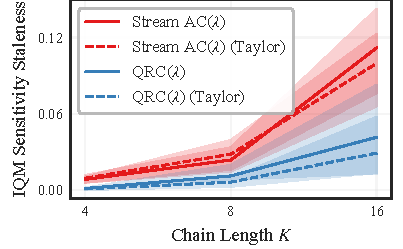
\includegraphics[width=\linewidth]{plots/staleness/sensitivity_staleness.pdf}
        \caption{RTRL sensitivity staleness on KMemoryChain. Relative $\ell_2$ distance between the online sensitivity matrix $\tilde{\boldsymbol{S}}_t$ and its recomputed reference $\boldsymbol{S}_t^\ast$, $\lVert \tilde{\boldsymbol{S}}_t - \boldsymbol{S}_t^\ast \rVert_2 / \lVert \boldsymbol{S}_t^\ast \rVert_2$,
over different chain lengths.}
        \label{fig:staleness}
    \end{subfigure}
    \hfill
    \begin{subfigure}[t]{0.49\linewidth}
        \centering
        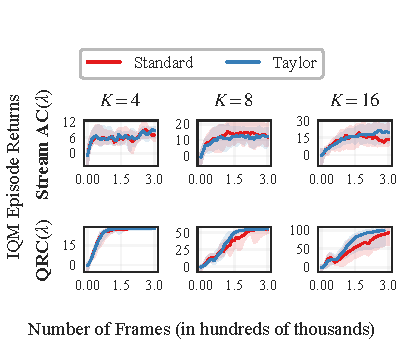
\includegraphics[width=\linewidth]{plots/staleness/episode_returns.pdf}
        \caption{IQM episodic return over 5 seeds with shaded standard error on different chain lengths of KMemoryChain.}
        \label{fig:stale_returns}
    \end{subfigure}
\end{figure}

\paragraph{Staleness metric.}
At every training step we maintain a buffer of the observations from the current episode. To form a reference, we replay the buffer forward from the saved initial state using the \emph{current} parameters $\boldsymbol{\psi}_t$, recomputing what the sensitivity would be if every immediate Jacobian in the episode had been evaluated at $\boldsymbol{\psi}_t$ rather than at the parameters in force when it was originally injected. The staleness reported is the $\ell_2$ distance between the live sensitivity carried by the algorithm and this recomputed reference. 

\paragraph{Result.}
Figure~\ref{fig:staleness} reports the IQM sensitivity staleness on KMemoryChain
as a function of the memory credit-assignment horizon $K$. Staleness rises
with $K$ across all four configurations, remaining near zero at $K{=}4$ and
growing through $K{=}8$ to its peak at $K{=}16$. This $K$-dependence is consistent
with the $(1-\rho)^{-2}$ scaling of the steady-state bound in
Equation~\eqref{eq:err_bound}: longer credit-assignment horizons require the
recurrence to retain memory over more steps, raising the effective contraction
constant and amplifying the bound.

The two algorithms differ in absolute staleness level: stream RAC($\lambda$)
staleness is consistently higher than RQRC($\lambda$) staleness and grows more
steeply with $K$. We attribute this gap to the optimizer rather than the
algorithm. Stream RAC($\lambda$) uses ObGD~\citep{elsayed2024streaming} with
base step size $\alpha=1$, which is scaled down only when the
effective-step-size threshold is violated and otherwise drives large per-step
parameter updates. RQRC($\lambda$), by contrast, uses plain SGD with fixed
learning rates of $10^{-4}$ for the Q-network and $10^{-5}$ for the auxiliary
$h$-network, two to three orders of magnitude smaller than the \emph{nominal} ObGD step, though
Appendix~\ref{sec:stepsize-analysis} measures ObGD's \emph{effective} step on masked Hopper at
around $10^{-4}$, the same order as RQRC($\lambda$)'s; the mechanism we suggest here is
therefore not established by the step sizes alone. Because the steady-state bound in Equation~\eqref{eq:err_bound} scales
linearly with the per-step parameter update magnitude $\eta G$, the larger
ObGD updates translate directly into proportionally larger steady-state
staleness. The Taylor correction reduces staleness across both algorithms,
with the largest absolute reduction at $K{=}16$ where the uncorrected
staleness is largest and the leading-order term predicted by
Equation~\eqref{eq:err_recur} dominates. At $K{=}4$ the corrected and
uncorrected variants are essentially indistinguishable, leaving little
headroom for a first-order correction to act on.

Figure~\ref{fig:stale_returns} reports the corresponding IQM episodic returns
across training for each $(\text{algorithm}, K)$ cell. The Taylor correction
does not degrade learning at any $K$, and at $K{=}4$ and $K{=}8$ it tracks the
standard sensitivity throughout training. At $K{=}16$, where the standard
sensitivity incurs the largest staleness, the Taylor correction appears to
learn faster and produce a more stable training curve, providing downstream
evidence that the staleness reductions in Figure~\ref{fig:staleness} translate
into improved credit assignment in the regime where the bound is tightest.
Taken together, streaming RTRL staleness stays bounded under sustained
credit-assignment load, scales with $K$ in the direction the bound predicts,
and tightens under the Taylor correction in the regime where the leading-order
term dominates.

\section{Staleness error bound for the \gls{rtrl} sensitivity matrix}
\label{sec:staleness-proof}

In the nonlinear setting, the \gls{rtrl} sensitivity matrix maintained by an
\gls{rtu} layer incurs a \emph{staleness error}: immediate Jacobians
accumulated at earlier steps were evaluated at parameters that the
optimizer has since moved away from. We bound this error and give a
second-order correction that reduces it from $\mathcal{O}(\eta)$ to
$\mathcal{O}(\eta^2)$.

\subsection{Setup and assumptions}
\label{sec:staleness-setup}

For a recurrent network $\boldsymbol{h}_t = \boldsymbol{f}(\boldsymbol{h}_{t-1}, \boldsymbol{x}_t; \boldsymbol{\psi})$ with state-to-state
Jacobian $\boldsymbol{J}_t = \partial \boldsymbol{h}_t / \partial \boldsymbol{h}_{t-1}$ and immediate Jacobian
$\boldsymbol{I}_t(\boldsymbol{\psi}) = \partial \boldsymbol{h}_t / \partial \boldsymbol{\psi}$, \gls{rtrl} maintains the sensitivity
matrix
\begin{equation}
    \boldsymbol{S}_t \;=\; \boldsymbol{J}_t\, \boldsymbol{S}_{t-1} \;+\; \boldsymbol{I}_t.
\end{equation}
Let $\boldsymbol{\psi}_t \in \mathbb{R}^p$ denote the recurrent parameters in force at
step $t$. The \emph{stale sensitivity matrix} maintained by the online
algorithm is
\begin{equation}
    \tilde{\boldsymbol{S}}_t \;=\; \boldsymbol{J}_t\, \tilde{\boldsymbol{S}}_{t-1} \;+\; \boldsymbol{I}_t(\boldsymbol{\psi}_t)
    \;=\; \sum_{k=0}^{t} \left(\prod_{j=k+1}^{t} \boldsymbol{J}_j\right) \boldsymbol{I}_k(\boldsymbol{\psi}_k),
\end{equation}
where the immediate Jacobian injected at step $k$ was evaluated at the
parameters $\boldsymbol{\psi}_k$ in force at that step. The \emph{ideal sensitivity
matrix}, which re-evaluates each historical immediate Jacobian at the
current parameters, is
\begin{equation}
    \boldsymbol{S}_t^\ast \;=\; \sum_{k=0}^{t} \left(\prod_{j=k+1}^{t} \boldsymbol{J}_j\right) \boldsymbol{I}_k(\boldsymbol{\psi}_t).
\end{equation}
The staleness error is $E_t = \|\boldsymbol{S}_t^\ast - \tilde{\boldsymbol{S}}_t\|$.

\paragraph{Assumptions.}
\begin{itemize}
    \item[(A1)] \textbf{Non-expansion.} $\|\boldsymbol{J}_t\| \le \rho \le 1$ uniformly in
    $t$.\footnote{For an \gls{rtu} layer with
    $\boldsymbol{\Lambda} = \mathrm{diag}(r_k e^{i\theta_k})$ the constant is
    $\rho = \max_k r_k$, kept at most one by the standard \gls{rtu}
    parameterization. A gated recurrence that learns to retain its state
    approaches the boundary $\rho = 1$, which the steady-state argument below
    excludes and the finite-horizon bound of
    Appendix~\ref{sec:staleness-finite} admits.}
    \item[(A2)] \textbf{Bounded updates.}
    $\|\boldsymbol{\psi}_t - \boldsymbol{\psi}_{t-1}\| \le \eta G$ for all $t$, where $\eta$ is a
    step size and $G$ bounds the per-step update magnitude.
    \item[(A3)] \textbf{Lipschitz immediate Jacobian.} The map
    $\boldsymbol{\psi} \mapsto \boldsymbol{I}_t(\boldsymbol{\psi})$ is Lipschitz with constant $L_I$,
    uniformly in $t$:
    $\|\boldsymbol{I}_t(\boldsymbol{\psi}) - \boldsymbol{I}_t(\boldsymbol{\psi'})\| \le L_I \|\boldsymbol{\psi} - \boldsymbol{\psi'}\|$.
    \item[(A4)] \textbf{Bounded magnitude.}
    $\|\boldsymbol{I}_t(\boldsymbol{\psi})\| \le M_I$ uniformly.
\end{itemize}

\paragraph{Bound on the sensitivity matrix.}
Taking norms in the stale recursion and applying the triangle inequality,
$\|\tilde{\boldsymbol{S}}_t\| \le \rho \|\tilde{\boldsymbol{S}}_{t-1}\| + M_I$,
which unrolls to the geometric steady-state bound
$\|\tilde{\boldsymbol{S}}_t\| \le M_I / (1 - \rho)$.

\paragraph{Error recurrence.}
Expanding $\boldsymbol{S}_{t+1}^\ast$ and $\tilde{\boldsymbol{S}}_{t+1}$, the injection at step $t+1$
cancels because both contain $\boldsymbol{I}_{t+1}(\boldsymbol{\psi}_{t+1})$. Adding and
subtracting $\boldsymbol{I}_k(\boldsymbol{\psi}_t)$ inside the bracket of the resulting
difference and factoring out the leading Jacobian $\boldsymbol{J}_{t+1}$,
\begin{equation}
    \boldsymbol{S}_{t+1}^\ast - \tilde{\boldsymbol{S}}_{t+1}
    \;=\; \boldsymbol{J}_{t+1}\!\sum_{k=0}^{t} \left(\prod_{j=k+1}^{t} \boldsymbol{J}_j\right)\!
    \bigl[\boldsymbol{I}_k(\boldsymbol{\psi}_{t+1}) - \boldsymbol{I}_k(\boldsymbol{\psi}_t)\bigr]
    \;+\; \boldsymbol{J}_{t+1}\bigl(\boldsymbol{S}_t^\ast - \tilde{\boldsymbol{S}}_t\bigr).
\end{equation}
Taking norms, applying (A1) to each product of Jacobians, applying (A2)
and (A3) to the freshly injected term, and bounding the geometric sum by
$1/(1-\rho)$,
\begin{equation}
    E_{t+1} \;\le\; \rho \cdot \frac{L_I\, \eta\, G}{1 - \rho}
    \;+\; \rho\, E_t.
    \label{eq:err_recur}
\end{equation}
This is a first-order linear recurrence with contraction factor
$\rho < 1$ and constant driving term. The transient $\rho^t E_0$
vanishes and the geometric series converges, yielding the steady-state
bound
\begin{equation}
    E_\infty \;\le\; \frac{\rho\, L_I\, G\, \eta}{(1 - \rho)^2}.
    \label{eq:err_bound}
\end{equation}

\paragraph{Periodic updates.}
If $\boldsymbol{\psi}$ is held fixed for $m$ steps between updates, the staleness
injected at each update decays by $\rho^m$ before the next, sharpening
the bound to
\begin{equation}
    E_\infty \;\le\;
    \frac{\rho\, L_I\, G\, \eta}{(1 - \rho)(1 - \rho^m)}.
\end{equation}
Since $1 - \rho^m \ge 1 - \rho$ for $m \ge 1$, periodic updates strictly
reduce the steady-state staleness.

\subsection{A finite-horizon bound without contraction}
\label{sec:staleness-finite}

The steady-state bound \eqref{eq:err_bound} requires $\rho < 1$ and diverges as
$\rho \to 1$. This excludes the case of interest for a gated recurrence that
learns to retain its state, where the retention factor of the units carrying the
signal approaches one. The episodic setting, however, bounds the accumulation
horizon by the episode length, so no contraction is needed if the error is
bounded over a finite horizon rather than in steady state.

Fix an episode of length $T$ and write $n = T - k$ for the lag of the
contribution injected at step $k$. Telescoping (A2) gives
$\|\boldsymbol{\psi}_T - \boldsymbol{\psi}_k\| \le \eta G (T-k)$, so applying (A3) to each
term of the difference between the ideal and stale matrices, and (A1) to each
product of Jacobians,
\begin{equation}
    E_T
    \;=\; \Bigl\| \sum_{k=0}^{T} \Bigl(\prod_{j=k+1}^{T} \boldsymbol{J}_j\Bigr)
      \bigl[\boldsymbol{I}_k(\boldsymbol{\psi}_T) - \boldsymbol{I}_k(\boldsymbol{\psi}_k)\bigr] \Bigr\|
    \;\le\; L_I\, \eta\, G \sum_{n=0}^{T} n\, \rho^{\,n},
    \label{eq:err_finite}
\end{equation}
which is finite for every $\rho \le 1$ and every finite $T$. Evaluating the sum,
\begin{equation}
    E_T \;\le\; L_I\, \eta\, G \,
    \frac{\rho\bigl(1 - (T+1)\rho^{\,T} + T \rho^{\,T+1}\bigr)}{(1-\rho)^2},
    \qquad \rho < 1,
\end{equation}
and taking $T \to \infty$ recovers \eqref{eq:err_bound}, so the finite-horizon
bound strictly generalises the steady-state one. At the boundary $\rho = 1$ the
sum evaluates to $T(T+1)/2$ and
\begin{equation}
    E_T \;\le\; \tfrac{1}{2}\, L_I\, \eta\, G\, T (T+1),
    \label{eq:err_rho_one}
\end{equation}
so a recurrence that retains its state perfectly still incurs staleness that is
bounded on any finite episode, growing at most quadratically in its length rather
than diverging. The two factors of $T$ have distinct origins: one counts the
contributions accumulated in the sensitivity matrix, and one measures how far the
parameters have moved since the oldest of them was injected.

\paragraph{Remark.} The bound \eqref{eq:err_finite} sums the magnitudes of the
per-step errors and is therefore tight only when those errors align. When the
increments $\boldsymbol{I}_k(\boldsymbol{\psi}_T) - \boldsymbol{I}_k(\boldsymbol{\psi}_k)$ are
not systematically aligned across $k$, their sum grows more slowly than the sum
of their norms, and the dependence on $T$ is correspondingly weaker.

\subsection{A first-order Taylor-trace correction}
\label{sec:staleness-correction}

The leading-order term in the error recurrence~\eqref{eq:err_recur} is
the freshly injected staleness
$\boldsymbol{I}_k(\boldsymbol{\psi}_{t+1}) - \boldsymbol{I}_k(\boldsymbol{\psi}_t)$. A first-order Taylor expansion in
$\boldsymbol{\psi}$ gives
\begin{equation}
    \boldsymbol{I}_k(\boldsymbol{\psi}_t) \;\approx\; \boldsymbol{I}_k(\boldsymbol{\psi}_{t-1})
    \;+\; \left.\frac{\partial \boldsymbol{I}_k}{\partial \boldsymbol{\psi}}\right|_{\boldsymbol{\psi}_{t-1}}\!\!
    \Delta\boldsymbol{\psi}_{t-1},
\end{equation}
where $\Delta\boldsymbol{\psi}_{t-1} = \boldsymbol{\psi}_t - \boldsymbol{\psi}_{t-1}$. Substituting into
$\boldsymbol{S}_t^\ast$ and grouping the second-order factors into an auxiliary
accumulator
\begin{equation}
    \boldsymbol{\Omega}_t \;=\; \boldsymbol{J}_t\, \boldsymbol{\Omega}_{t-1}
    \;+\; \left.\frac{\partial \boldsymbol{I}_t}{\partial \boldsymbol{\psi}}\right|_{\boldsymbol{\psi}_t}
\end{equation}
yields a corrected update
\begin{equation}
    \boldsymbol{S}_t \;=\; \boldsymbol{J}_t\,\bigl(\boldsymbol{S}_{t-1} + \boldsymbol{\Omega}_{t-1}\, \Delta\boldsymbol{\psi}_{t-1}\bigr)
    \;+\; \boldsymbol{I}_t(\boldsymbol{\psi}_t).
\end{equation}
The additive term $\boldsymbol{J}_t\, \boldsymbol{\Omega}_{t-1}\, \Delta\boldsymbol{\psi}_{t-1}$ neutralizes
the leading-order staleness injection, reducing the residual error from
$\mathcal{O}(\|\Delta\boldsymbol{\psi}\|)$ to $\mathcal{O}(\|\Delta\boldsymbol{\psi}\|^2)$.

Storing $\boldsymbol{\Omega}_t$ exactly is intractable: since $\boldsymbol{I}_t$ has shape
$|h| \times p$, $\boldsymbol{\Omega}_t$ is a rank-three tensor of shape
$|h| \times p \times p$ requiring $\mathcal{O}(|h|\, p^2)$ memory. A
parameter-wise diagonal approximation,
\begin{equation}
    \boldsymbol{\omega}_t \;=\; \boldsymbol{J}_t\, \boldsymbol{\omega}_{t-1}
    \;+\; \mathrm{diag}_{\boldsymbol{\psi}}\!\left(\frac{\partial \boldsymbol{I}_t}{\partial \boldsymbol{\psi}}\right),
    \quad
    \boldsymbol{S}_t \;=\; \boldsymbol{J}_t\,\bigl(\boldsymbol{S}_{t-1} + \boldsymbol{\omega}_{t-1} \odot \Delta\boldsymbol{\psi}_{t-1}\bigr)
    \;+\; \boldsymbol{I}_t(\boldsymbol{\psi}_t),
    \label{eq:taylor-diag}
\end{equation}
recovers the original space complexity of the \gls{rtrl} sensitivity,
where $\odot$ denotes the elementwise product along the parameter axis.

%%%%%%%%%%%%%%%%%%%%%%%%%%%%%%%%%%%%%%%%%%%%%%%%%%%%%%%%%%%%%%%%
%% NOTE: THIS MARKS THE END OF THE "MAIN TEXT"
%%%%%%%%%%%%%%%%%%%%%%%%%%%%%%%%%%%%%%%%%%%%%%%%%%%%%%%%%%%%%%%%

%%%%%%%%%%%%%%%%%%%%%%%%%%%%%%%%%%%%%%%%%%%%%%%%%%%%%%%%%%%%%%%%
%% Bibliography
%%%%%%%%%%%%%%%%%%%%%%%%%%%%%%%%%%%%%%%%%%%%%%%%%%%%%%%%%%%%%%%%

%% Acknowledgments withheld for double-blind review; restore before the camera-ready.
%% \subsubsection*{Acknowledgments}
%% Noah Farr is supported by the Konrad Zuse School of Excellence in Learning and Intelligent Systems (\textbf{\href{https://eliza.school/}{ELIZA}}) through the DAAD programme Konrad Zuse Schools of Excellence in Artificial Intelligence, sponsored by the Federal Ministry of Education and Research.


\end{document}
